%%
% This is an Overleaf template for presentations
% using the TUM Corporate Desing https://www.tum.de/cd
%
% For further details on how to use the template, take a look at our
% GitLab repository and browse through our test documents
% https://gitlab.lrz.de/latex4ei/tum-templates.
%
% The tumbeamer class is based on the beamer class.
% If you need further customization please consult the beamer class guide
% https://ctan.org/pkg/beamer.
% Additional class options are passed down to the base class.
%
% If you encounter any bugs or undesired behaviour, please raise an issue
% in our GitLab repository
% https://gitlab.lrz.de/latex4ei/tum-templates/issues
% and provide a description and minimal working example of your problem.
%%


\documentclass[
  english,            % define the document language (english, german)
  aspectratio=169,    % define the aspect ratio (169, 43)
  % handout=2on1,       % create handout with multiple slides (2on1, 4on1)
  % partpage=false,     % insert page at beginning of parts (true, false)
  % sectionpage=true,   % insert page at beginning of sections (true, false)
  11pt
]{tumbeamer}


% load additional packages
\usepackage{booktabs}
\usepackage{listings}
\usepackage{xcolor}
\usepackage{lmodern}
\usepackage{enumitem}
\usepackage[font=scriptsize]{caption}

\definecolor{codegreen}{rgb}{0,0.6,0}
\definecolor{codegray}{rgb}{0.5,0.5,0.5}
\definecolor{codepurple}{rgb}{0.58,0,0.82}
\definecolor{backcolour}{rgb}{0.95,0.95,0.92}

\lstdefinestyle{mystyle}{
    backgroundcolor=\color{backcolour},   
    commentstyle=\color{codegreen},
    keywordstyle=\color{magenta},
    numberstyle=\tiny\color{codegray},
    stringstyle=\color{codepurple},
    basicstyle=\ttfamily\footnotesize,
    breakatwhitespace=false,         
    breaklines=true,                 
    captionpos=b,                    
    keepspaces=true,                 
    numbers=left,                    
    numbersep=5pt,                  
    showspaces=false,                
    showstringspaces=false,
    showtabs=false,                  
    tabsize=2
}
% \lstset{style=mystyle}
\lstset{language=bash,
	,basicstyle=\ttfamily\tiny,
	keywordstyle=\color{blue}\ttfamily,
	stringstyle=\color{red}\ttfamily,
	commentstyle=\color{green}\ttfamily,
	morecomment=[l][\color{magenta}]{\#}
}


%\usepackage{hyperref}
%\usepackage{tabularx}

%\usepackage{listings}
%\usepackage{caption}
%\usepackage{subcaption}
%\usepackage{subfigure}
%\usepackage{algpseudocode,algorithm,algorithmicx}
%\usepackage{biblatex}
%\usepackage{cite}


% presentation metadata
\title{HPC-lab }
\subtitle{Final Project\\
	 CUDA-Aware MPI with UVA}
\author{Phuong Nguyen, Zirong Cai}

\institute{\theChairName\\\theDepartmentName\\\theUniversityName}
\date[8/11/2021]{November 8\textsuperscript{th}, 2021}

\footline{\insertauthor~|~\insertshorttitle~|~\insertshortdate}


% macro to configure the style of the presentation
\TUMbeamersetup{
  title page = TUM tower,         % style of the title page
  part page = TUM toc,            % style of part pages
  section page = TUM toc,         % style of section pages
  content page = TUM more space,  % style of normal content pages
  tower scale = 1.0,              % scaling factor of TUM tower (if used)
  headline = TUM threeliner,      % which variation of headline to use
  footline = TUM default,         % which variation of footline to use
  % configure on which pages headlines and footlines should be printed
  headline on = {title page},
  footline on = {every page, title page=false},
}

% available frame styles for title page, part page, and section page:
% TUM default, TUM tower, TUM centered,
% TUM blue default, TUM blue tower, TUM blue centered,
% TUM shaded default, TUM shaded tower, TUM shaded centered,
% TUM flags
%
% additional frame styles for part page and section page:
% TUM toc
%
% available frame styles for content pages:
% TUM default, TUM more space
%
% available headline options:
% TUM empty, TUM oneliner, TUM twoliner, TUM threeliner, TUM logothreeliner
%
% available footline options:
% TUM empty, TUM default, TUM infoline
\setlist[itemize]{label={\tiny\color{blue}$\blacksquare$}}%\textbullet}}

\begin{document}



\maketitle

\section{Introduction}
%%%%%%%%%%%%%%%%%%%%%%%%%%%%%%%%%%%%%%%%%%%%%%%%%%%%%%%%%%%%%%%%%%%%%%%%%%%%%%%

\begin{frame}[fragile]{SWE with CUDA - Current Implementation}
	\begin{minipage}[t]{0.4\textwidth}
		\begin{figure}
			\centering
			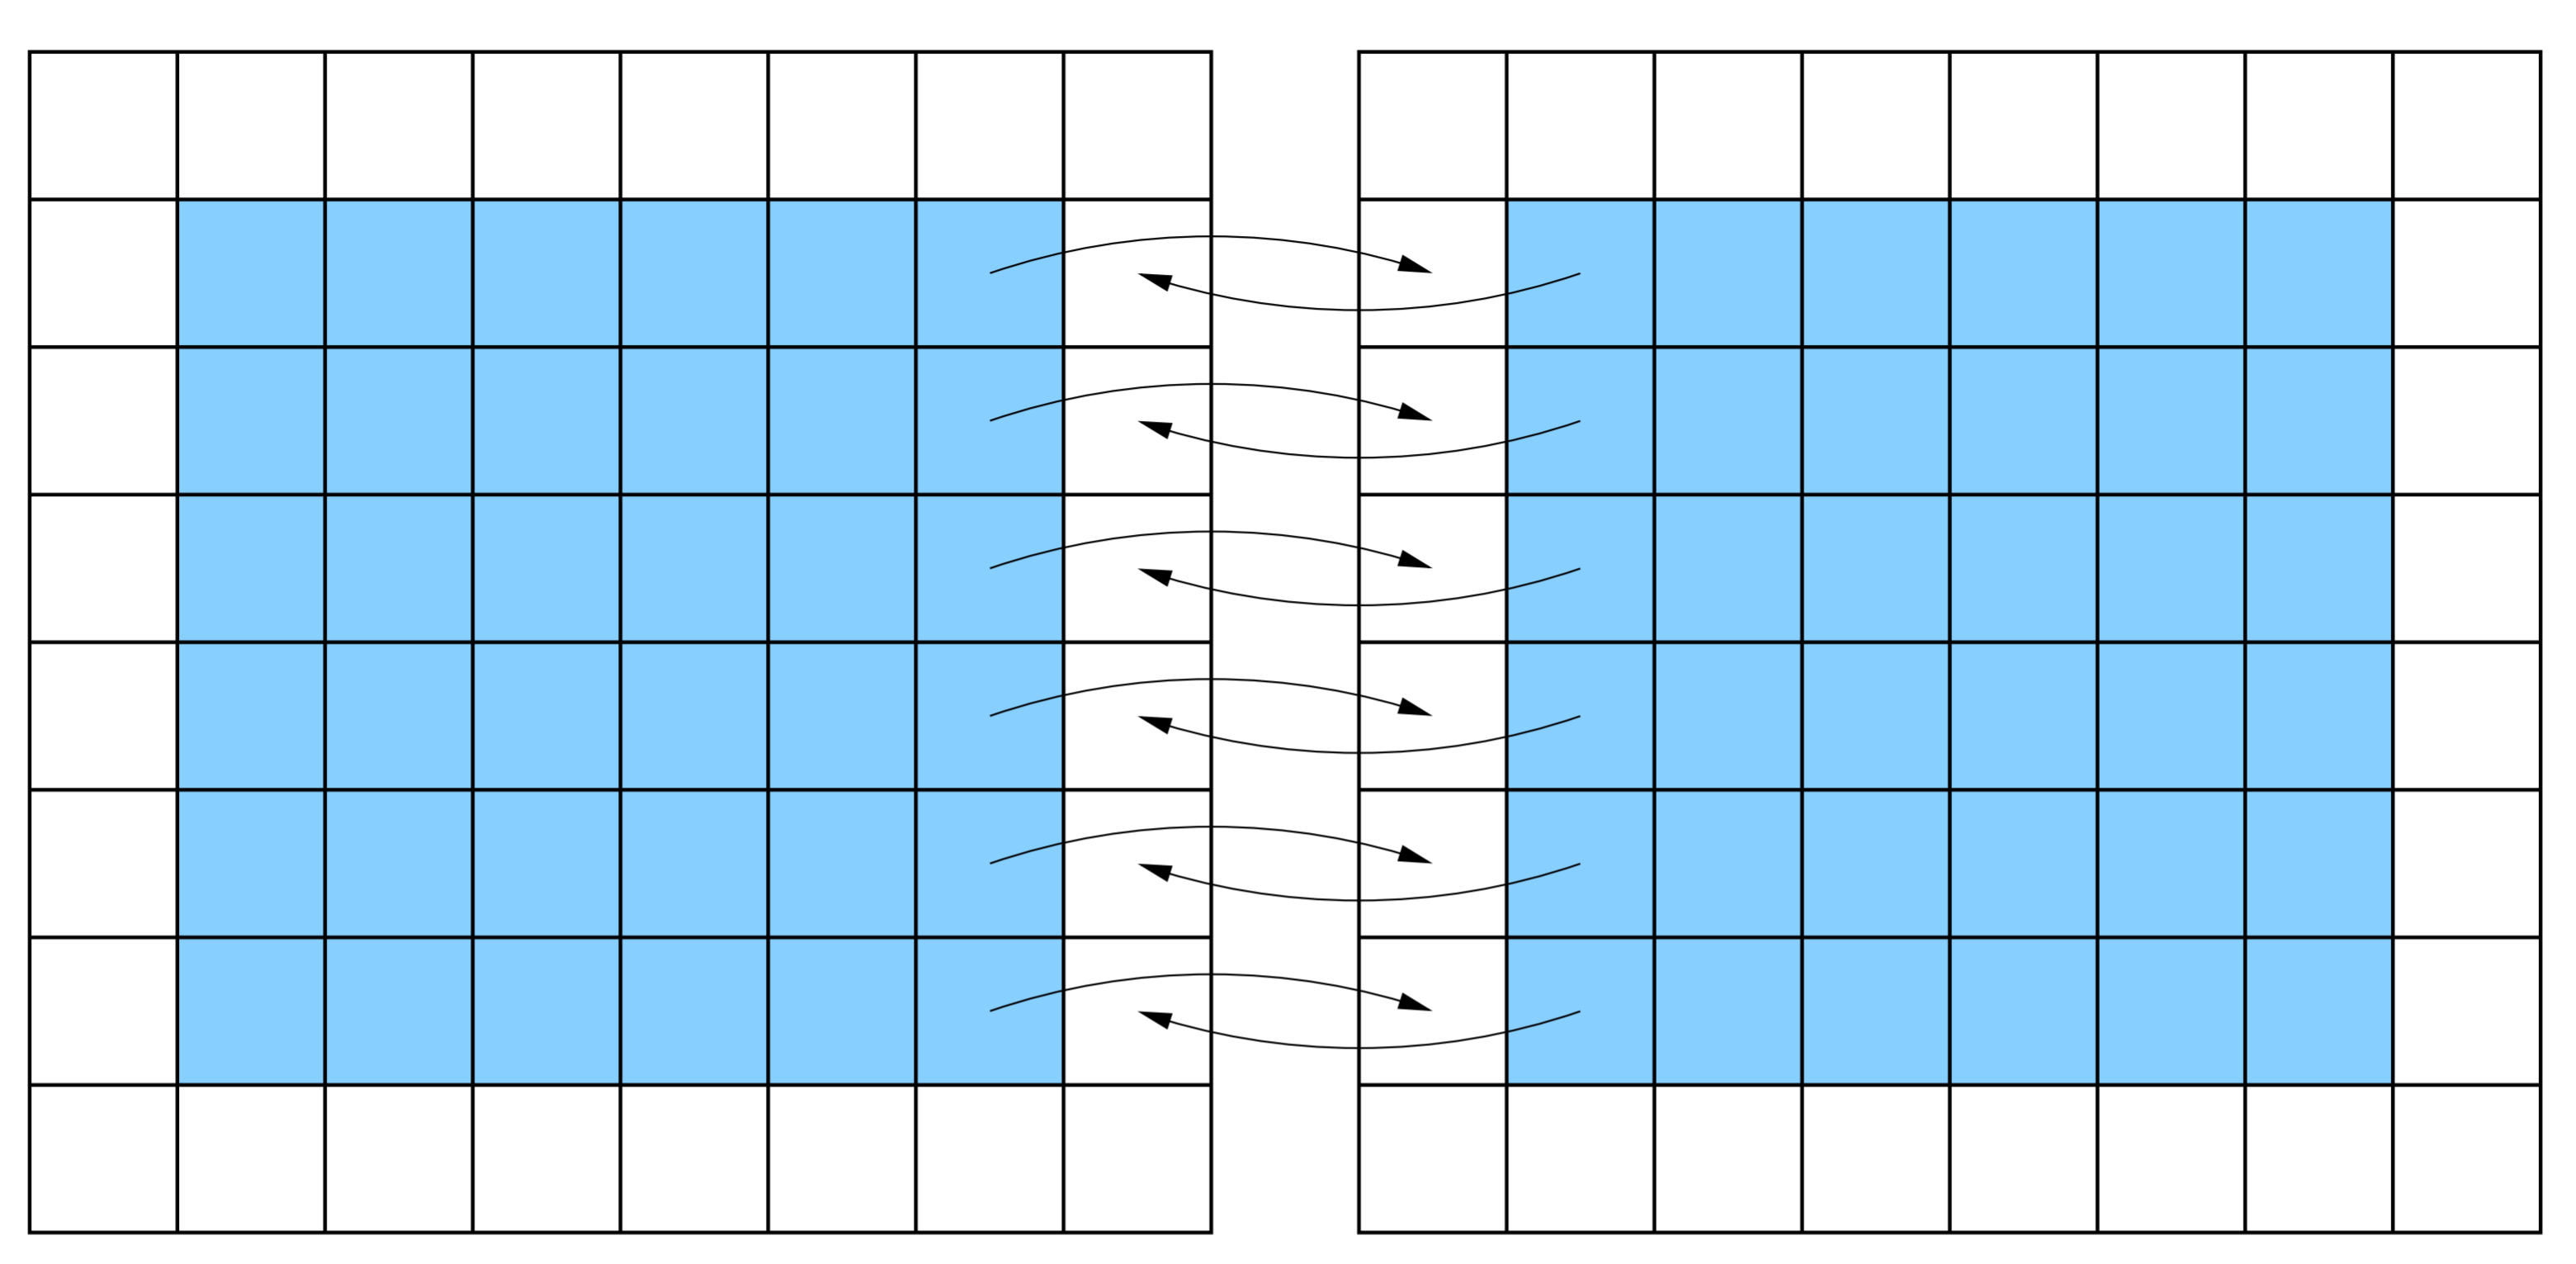
\includegraphics[width=\textwidth,keepaspectratio=true]{figs/2dgrid.png}
			\caption{Caption}
			\label{fig:my_label}
		\end{figure}
	\end{minipage}
	%
	\begin{minipage}[t]{0.04\textwidth}
	\end{minipage}
	%
	\begin{minipage}[t]{0.52\textwidth}
		%\fontsize{2}{1}
		\tiny
		\begin{lstlisting}[frame=single]
While () 
{
exchangeGhostLayers(); 		// On Host
setGhostLayer(); 
memcpy H-> D;
computeNumericalFluxes();		// On Device
MPI_Allreduce(&l_maxTimeStep, \
	&l_maxTimeGlobal, ...);
updateUnknowns(l_maxTimeGlobal);	// On Device
memcpy D-> H;
iteration++;
}
		\end{lstlisting}
	\end{minipage}
	%  synchGhostLayerAfterWrite(); 
	%  synchCopyLayerBeforeRead() 
	\begin{itemize}
		\item Allocate data on both Host and Device memory.
		\item Need to copy data between Host - Device explicitly. 
		\item Additional data structures are required for exchanging ghost layer with top \& bottom neighbors (\textit{topLayer}, \textit{bottomLayer}).
	\end{itemize}
	
\end{frame}

\begin{frame}{SWE CUDA with MPI}

\begin{columns}
    \begin{column}{0.45\textwidth}
    	\vskip-2em
    	\begin{figure}
    		\centering
    		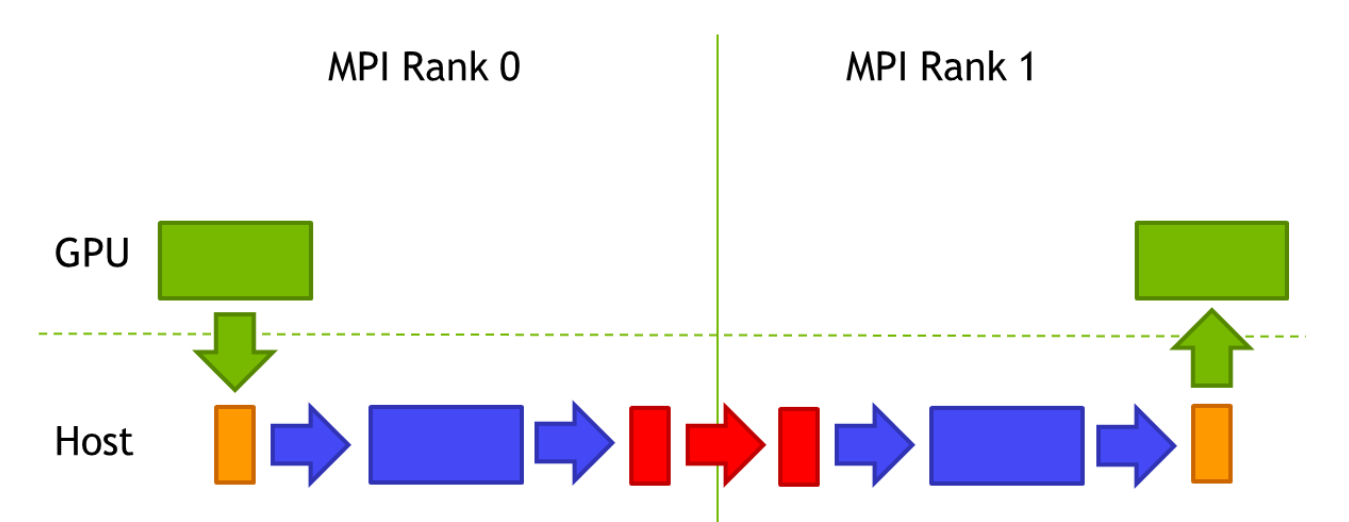
\includegraphics[width=\textwidth,keepaspectratio=true]{figs/cuda_scheme.png}
    	\end{figure}
    	\begin{columns}
    		\begin{column}{0.14\textwidth}
    		\end{column}
    	\begin{column}{0.85\textwidth}
    		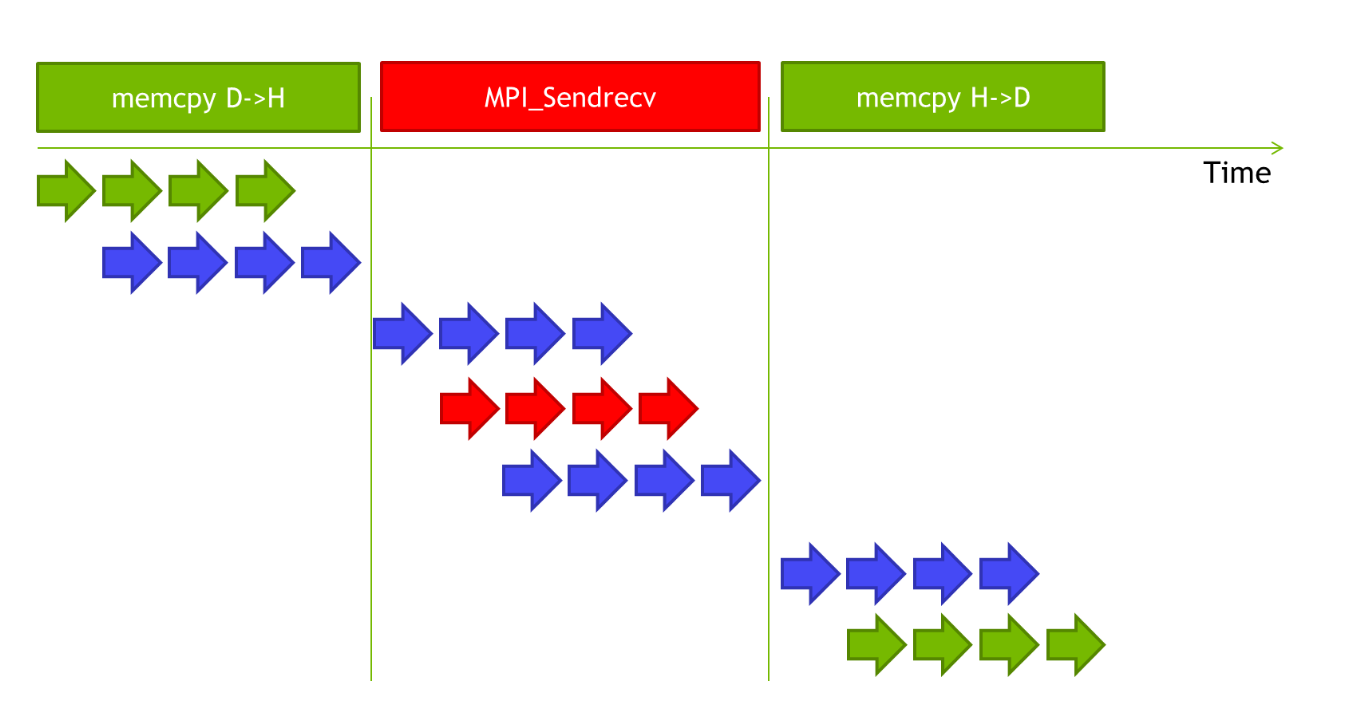
\includegraphics[width=\textwidth,keepaspectratio=true]{figs/cuda_scheme_time.png}
    	\end{column}
    	\end{columns}
    \end{column}
    \begin{column}{0.45\textwidth}
       
    \end{column}
\end{columns}

\end{frame}

%%%%%%%%%%%%%%%%%%%%%%%%%%%%%%%%%%%%%%%%%%%%%%%%%%%%%%%%%%%%%%%%%%%%%%%%%%%%%%%

\begin{frame}{CUDA Aware MPI}
\begin{columns}
	\begin{column}{0.45\textwidth}
		\vskip-2em
		\begin{figure}
			\centering
			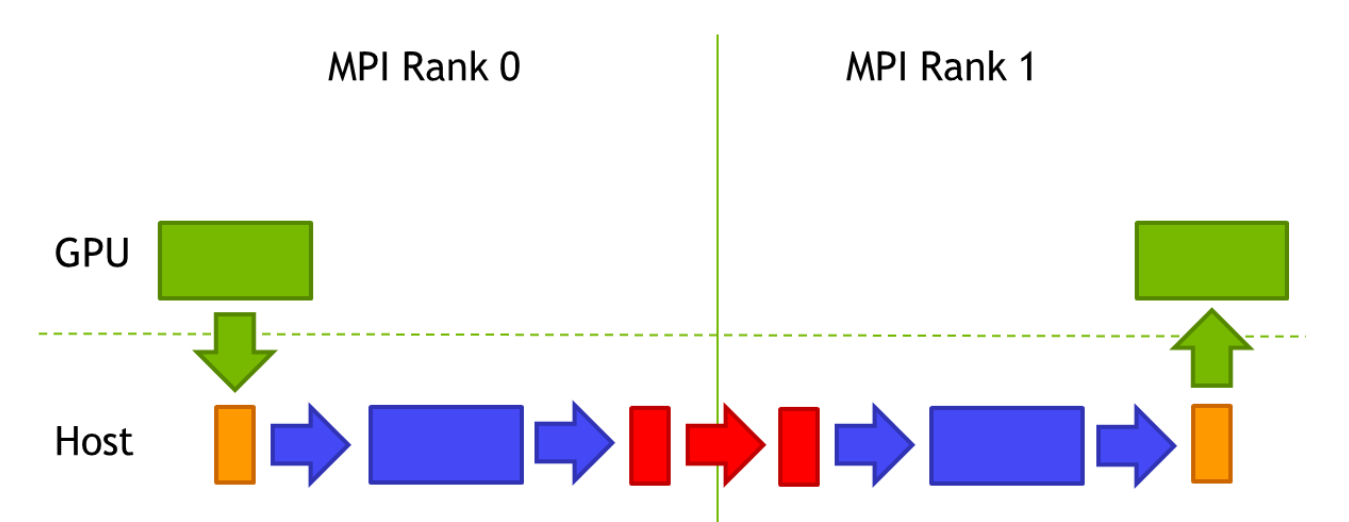
\includegraphics[width=\textwidth,keepaspectratio=true]{figs/cuda_scheme.png}
		\end{figure}
		\vskip-2em
		\begin{columns}
			\begin{column}{0.14\textwidth}
			\end{column}
			\begin{column}{0.85\textwidth}
				\begin{figure}
				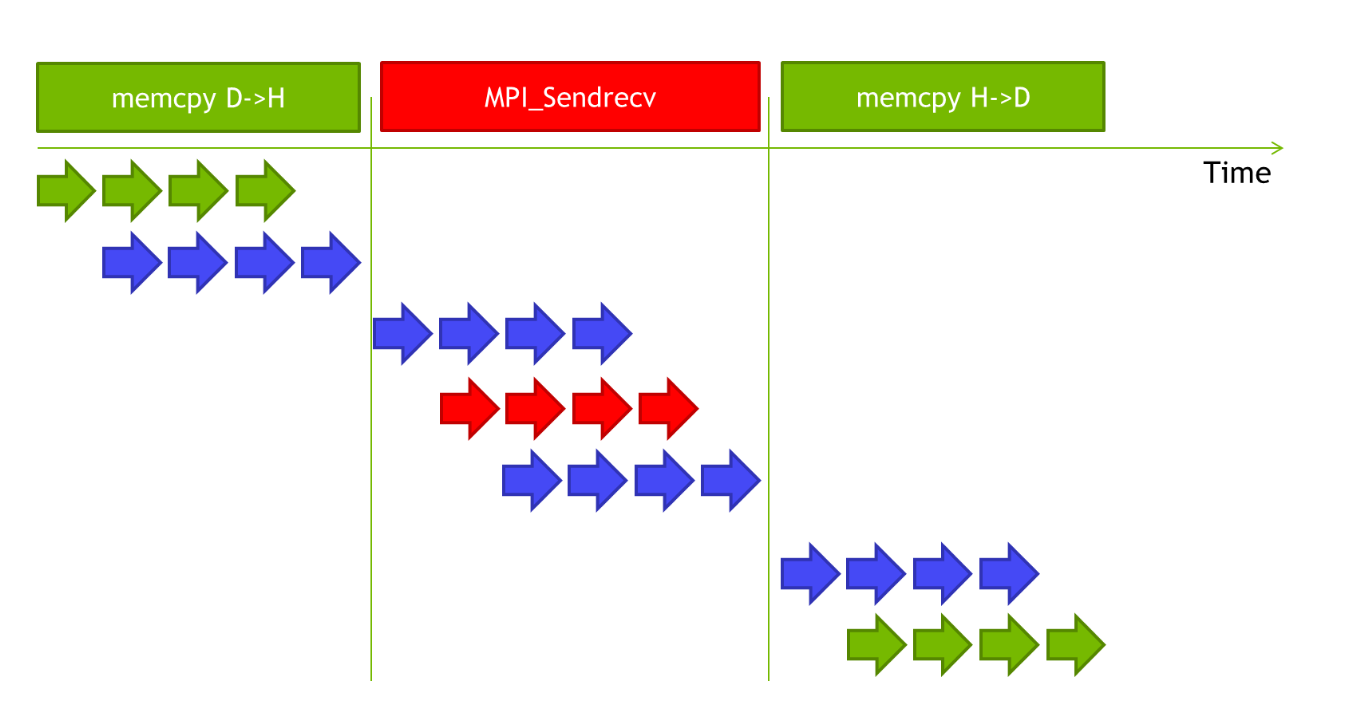
\includegraphics[width=\textwidth,keepaspectratio=true]{figs/cuda_scheme_time.png}
				\caption{CUDA MPI}
				\end{figure}
			\end{column}
		\end{columns}
	\end{column}

	\begin{column}{0.45\textwidth}
	\vskip-2em
	\begin{figure}
	\centering
	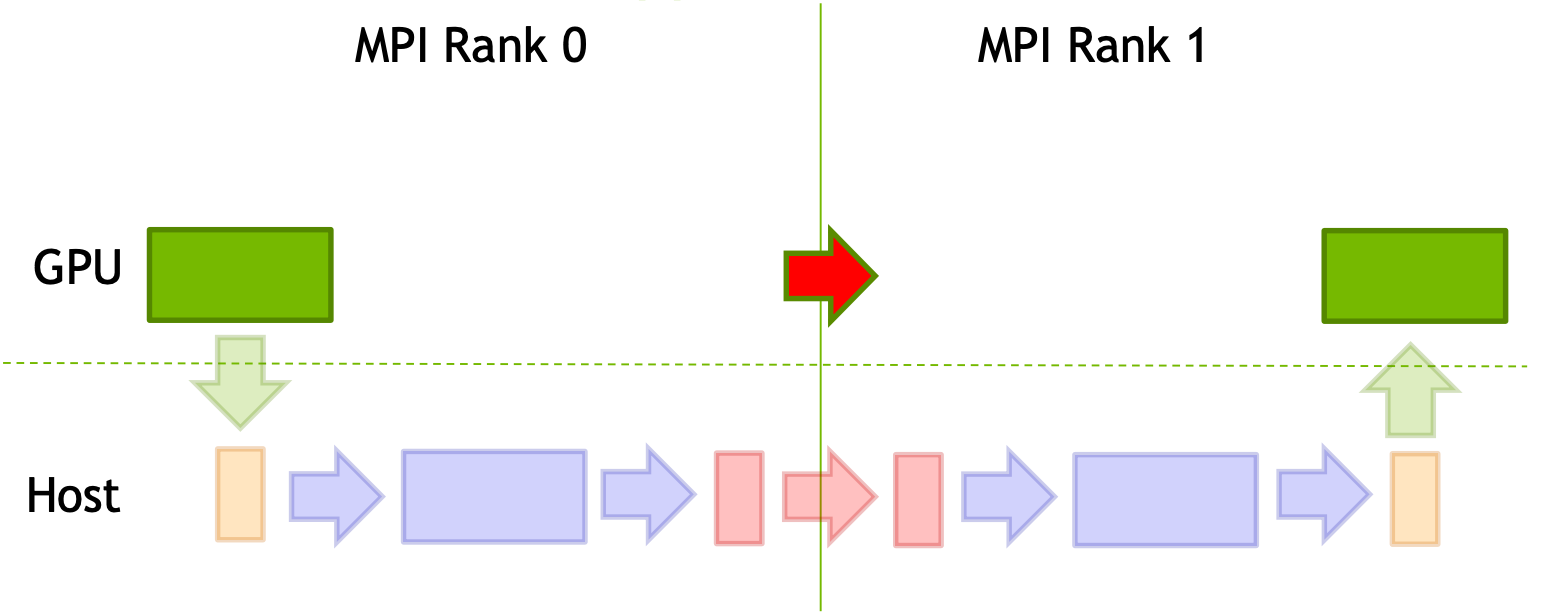
\includegraphics[width=\textwidth,keepaspectratio=true]{figs/GPUDirect_RDMA.png}
	\end{figure}
	\vskip-2em
	\begin{columns}
		\begin{column}{0.2\textwidth}
		\end{column}
		\begin{column}{0.8\textwidth}
				\begin{figure}
	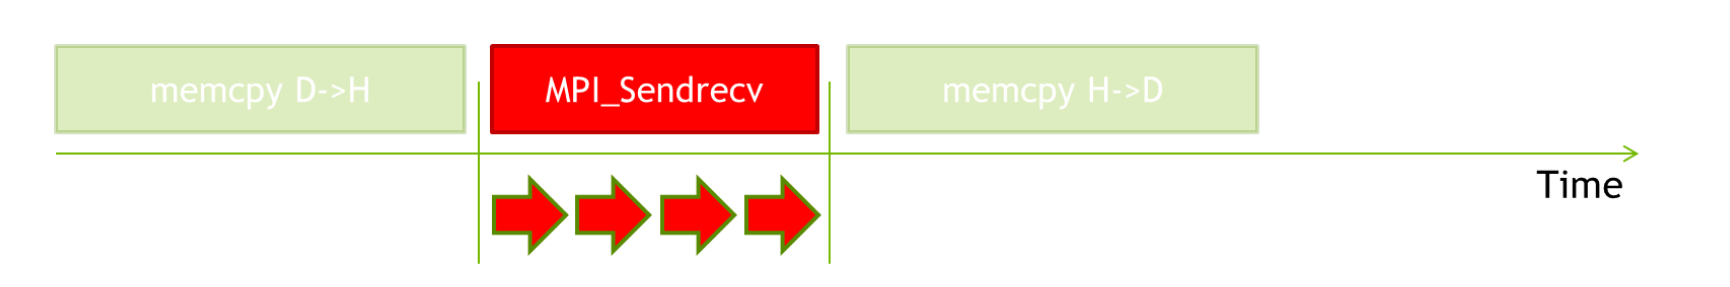
\includegraphics[width=\textwidth,keepaspectratio=true]{figs/cuda_aware_timeline.png}
	\vskip5.5em
	\caption{CUDA-Aware MPI}
		\end{figure}

	
		\end{column}
	\end{columns}
	\end{column}
\end{columns}
	
 \end{frame}

%%%%%%%%%%%%%%%%%%%%%%%%%%%%%%%%%%%%%%%%%%%%%%%%%%%%%%%%%%%%%%%%%%%%%%%%%%%%%%%

%\section{Theoretical Background}

\begin{frame}{Unified Memory}
    \begin{itemize}
        \item Unified Memory is a single memory address space accessible from any processor in a system.
        \item CUDA system software and/or the hardware takes care of migrating memory
    \end{itemize}
    \begin{figure}
        \centering
        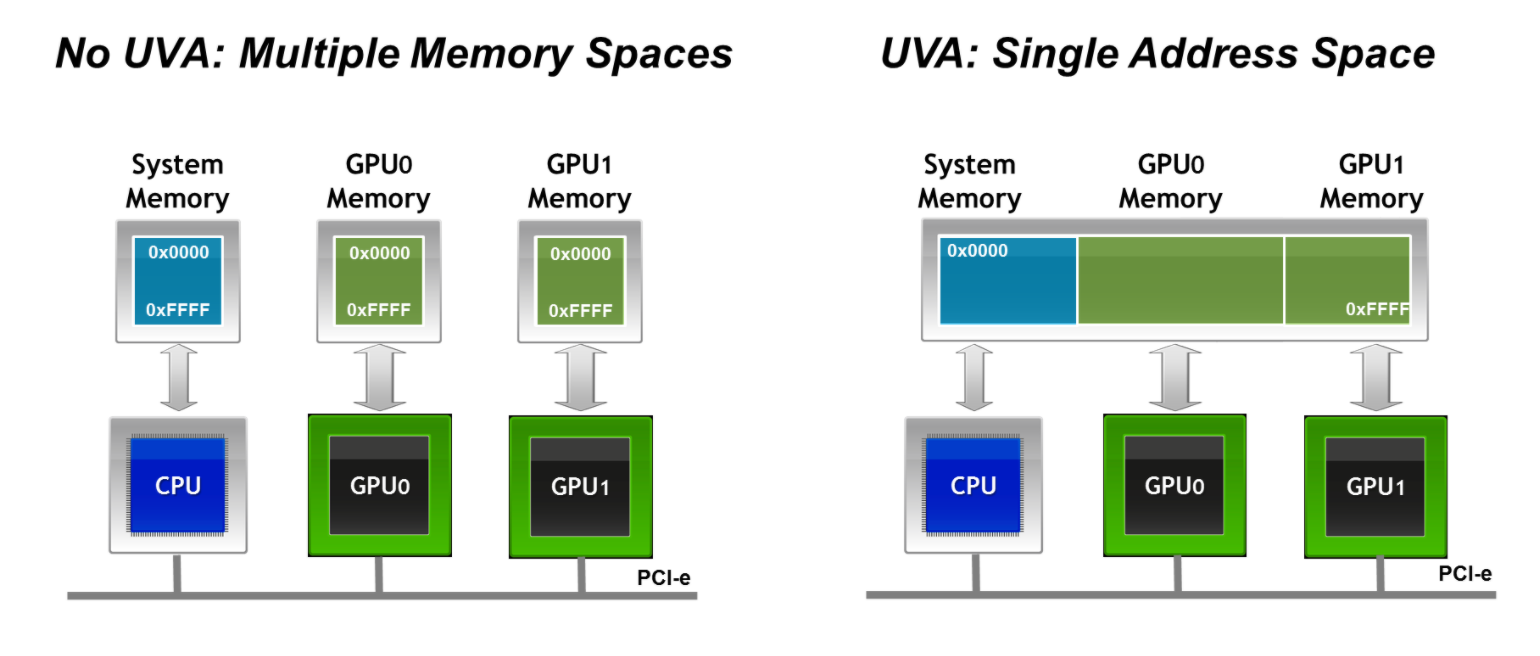
\includegraphics[width=.7\textwidth,height=.8\textheight,keepaspectratio=true]{figs/UnifiedMemoryCompare.png}
        \caption{No Unified Memory Vs. Unified Memory}
    \end{figure}
\end{frame}

%%%%%%%%%%%%%%%%%%%%%%%%%%%%%%%%%%%%%%%%%%%%%%%%%%%%%%%%%%%%%%%%%%%%%%%%%%%%%%%

%Add itemize to show 3 different GPUDirect:normal, p2p, rdma

\begin{frame}{GPUDiect}
	\vskip1em
 		NVIDIA GPUDirect technologies provide high-bandwidth, low-latency communications\\
 		with NVIDIA GPUs. 
        \begin{itemize}
            %\item GPUDirect
            \item GPUDirect P2P
            \item GPUDirect RDMA
        \end{itemize}

\begin{figure}
    \centering
    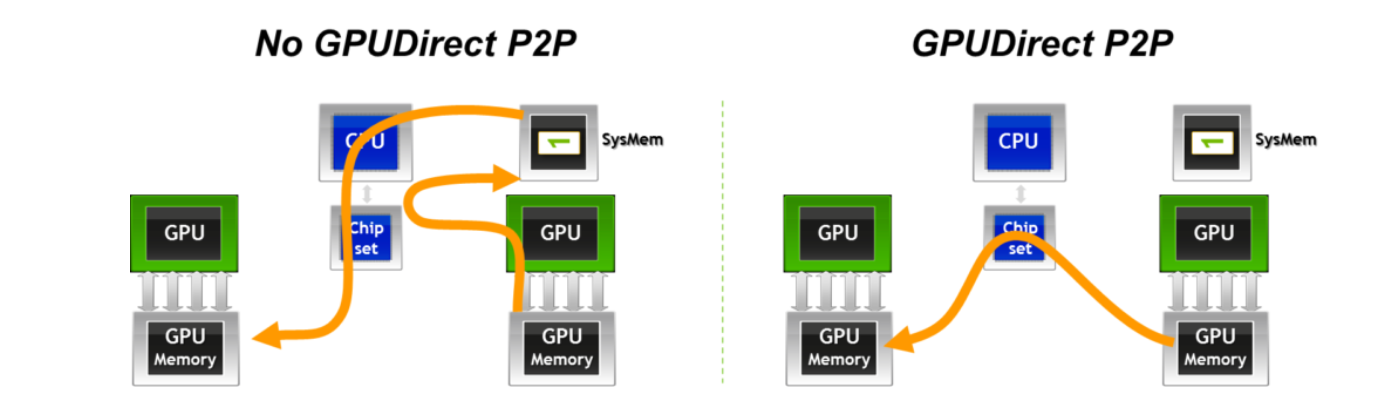
\includegraphics[width=.7\textwidth,height=.8\textheight,keepaspectratio=true]{figs/GPUDirectP2P.png}
    \caption{}
    %\label{fig:my_label}
\end{figure}
    
\end{frame}

%%%%%%%%%%%%%%%%%%%%%%%%%%%%%%%%%%%%%%%%%%%%%%%%%%%%%%%%%%%%%%%%%%%%%%%%%%%%%%%

\section{Implementation}






\begin{frame}{SWE with CUDA-Aware MPI}
\vfill
Implementing Unified Virtual Address (UVA):
  \begin{itemize}
  	\item \textit{h}, \textit{hv}, \textit{hu} are allocated on UVA.
  	\item Other helper variables for kernel functions: still on device memory. 
  	\item No explicit Copy data between Host - Device. 
  \end{itemize}
\vfill
MPI implementation:
	\begin{itemize}
		\item Taking UVA pointers.
		\item Pack data directly from the grid data (which is on UVA).
		\item For top/bottom layer exchange: strided data access is possible, using \\
		\textit{\footnotesize MPI\_Type\_vector(l\_nXLocal + 2, 1, l\_nYLocal + 2, MPI\_FLOAT, \&l\_mpiRow)};
	\end{itemize}

\vfill
\end{frame}

%%%%%%%%%%%%%%%%%%%%%%%%%%%%%%%%%%%%%%%%%%%%%%%%%%%%%%%%%%%%%%%%%%%%%%%%%%%%%%%

%\begin{frame}{MPI Communication}
    
%\end{frame}


%%%%%%%%%%%%%%%%%%%%%%%%%%%%%%%%%%%%%%%%%%%%%%%%%%%%%%%%%%%%%%%%%%%%%%%%%%%%%%%

%\begin{frame}{Bug Report}
    
    
%\end{frame}


%%%%%%%%%%%%%%%%%%%%%%%%%%%%%%%%%%%%%%%%%%%%%%%%%%%%%%%%%%%%%%%%%%%%%%%%%%%%%%%


\begin{frame}[fragile]{Error Test}
	\begin{columns}
		\begin{column}{0.4\textwidth}
			\vfill
		Error test implementation:
		\begin{itemize}
			\item \textit{-DENABLE\_TEST}: prints \textit{h} to an output file.
			\item \textit{test/error\_check.py}: calculates the absolute difference between 2 input data files.
			\item \textit{test/run\_test.sh}: executable script (compilation, runs, error check. 
		\end{itemize}
		\end{column}
		\begin{column}{0.5\textwidth}
		\tiny
		\begin{lstlisting}[frame=single,language=C++,caption={Parallel IO for printing \textit{h}}, captionpos=b]
// 2D subarray Datatype for MPI_File_set_view
MPI_Type_create_subarray(ndims,  gsizes,\
	lsizes, starts, MPI_ORDER_C,\
	MPI_FLOAT, &subarr_type);
...
// Datatype for printing data
MPI_Type_vector(l_nXLocal, l_nYLocal, \
	l_nYLocal + 2, MPI_FLOAT, &print_type);
...
MPI_File_open(MPI_COMM_WORLD, filename.c_str(),\
MPI_MODE_WRONLY + MPI_MODE_CREATE,\
MPI_INFO_NULL, &file);

MPI_File_set_view(file, 0, MPI_FLOAT, subarr_type,\
	"native", MPI_INFO_NULL);
MPI_File_write_all(file, &h_test[1][1], 1,\
	print_type, &status);
		
MPI_File_close(&file);
\end{lstlisting}
		\end{column}
	\end{columns}

\end{frame}

\begin{frame}{SWE-CUDA Issue (1)}
\begin{columns}
\begin{column}{0.45\textwidth}
	\begin{figure}[htpb]
		\centering
		\begin{subfigure}{.49\textwidth}
			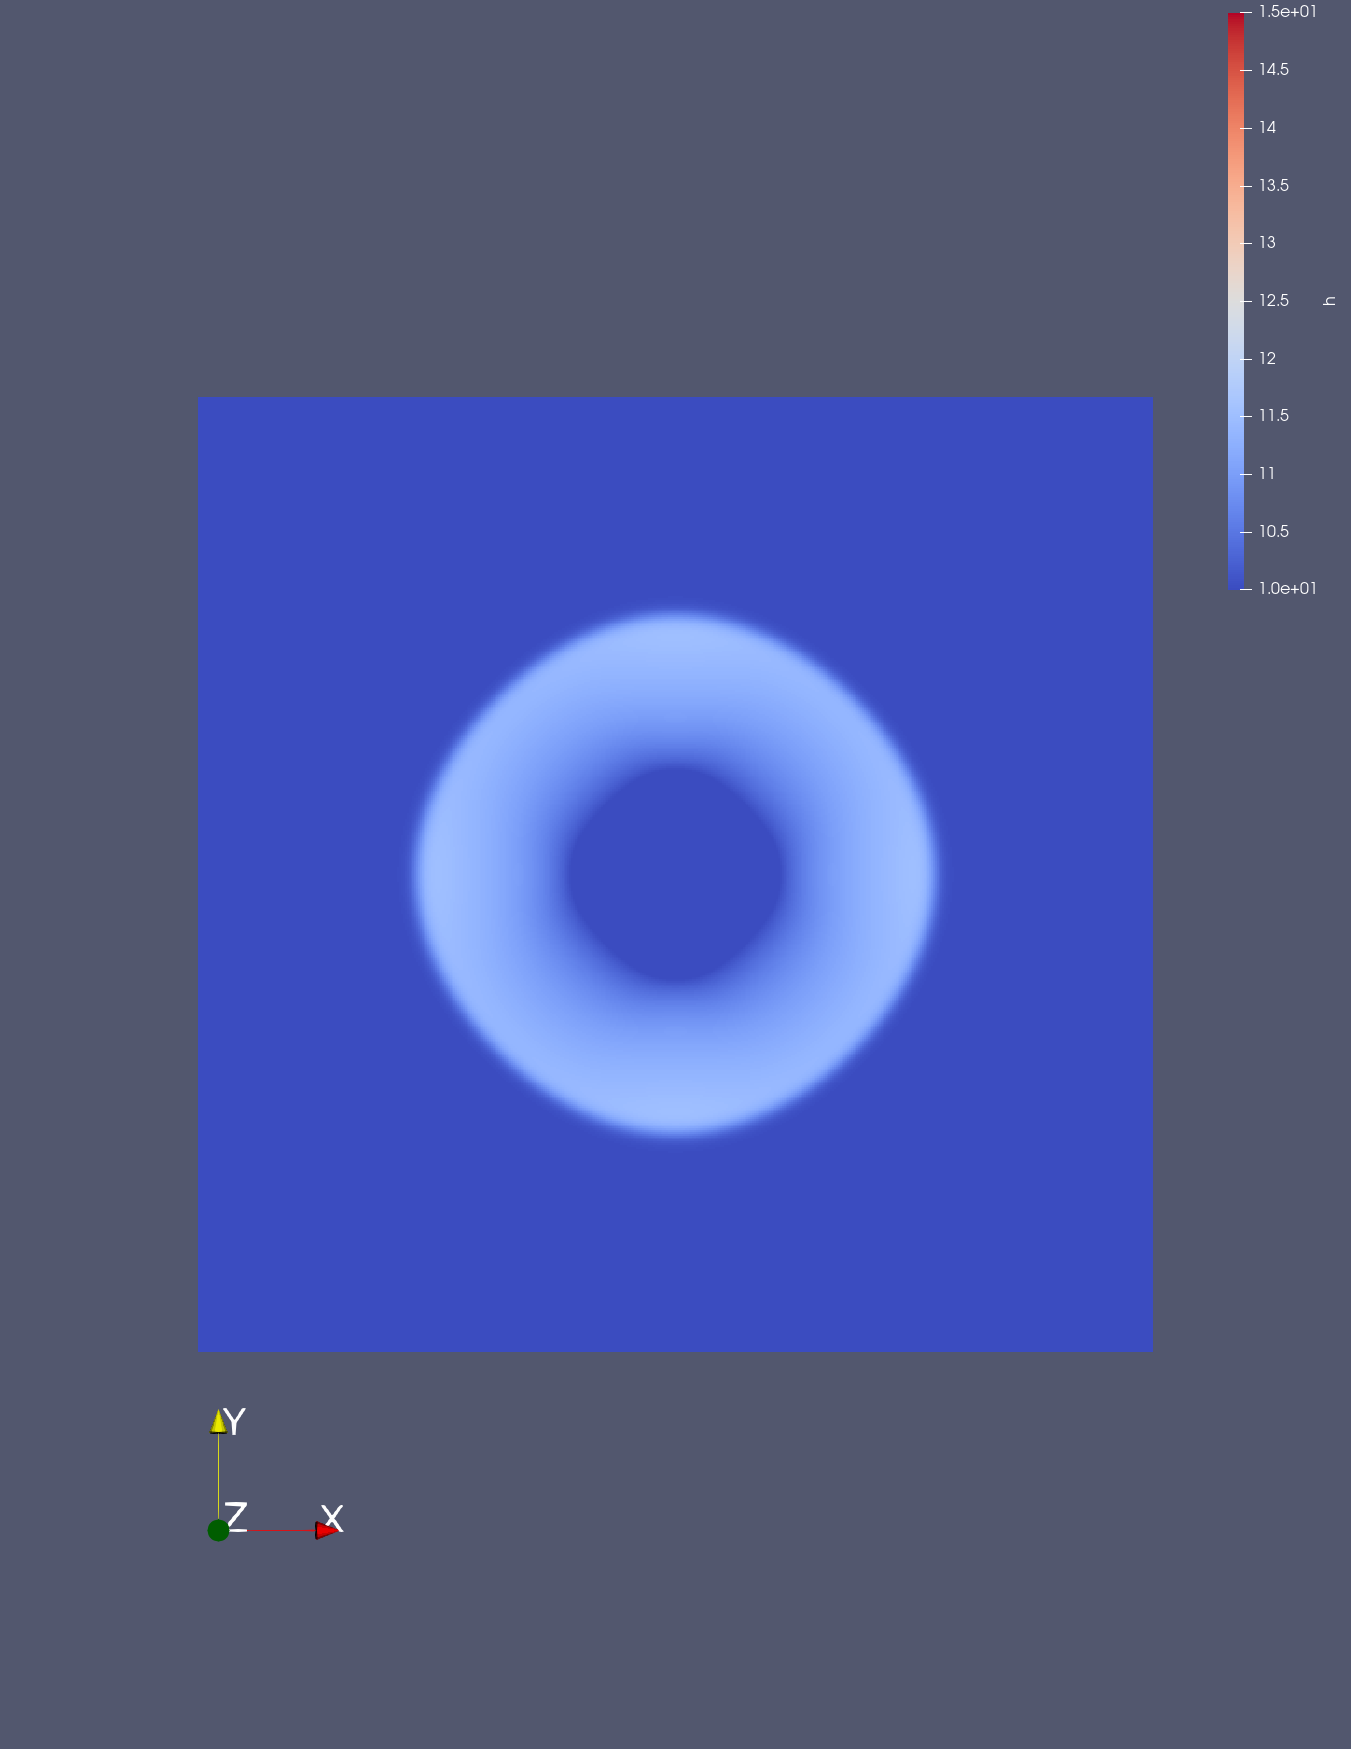
\includegraphics[width=\textwidth,keepaspectratio=true]{figs/1_validation_cuda_original_1mpi.png}
			\caption{1 MPI}
			\label{fig:1mpi}
		\end{subfigure}
		%
		\begin{subfigure}{.49\textwidth}
			\centering
			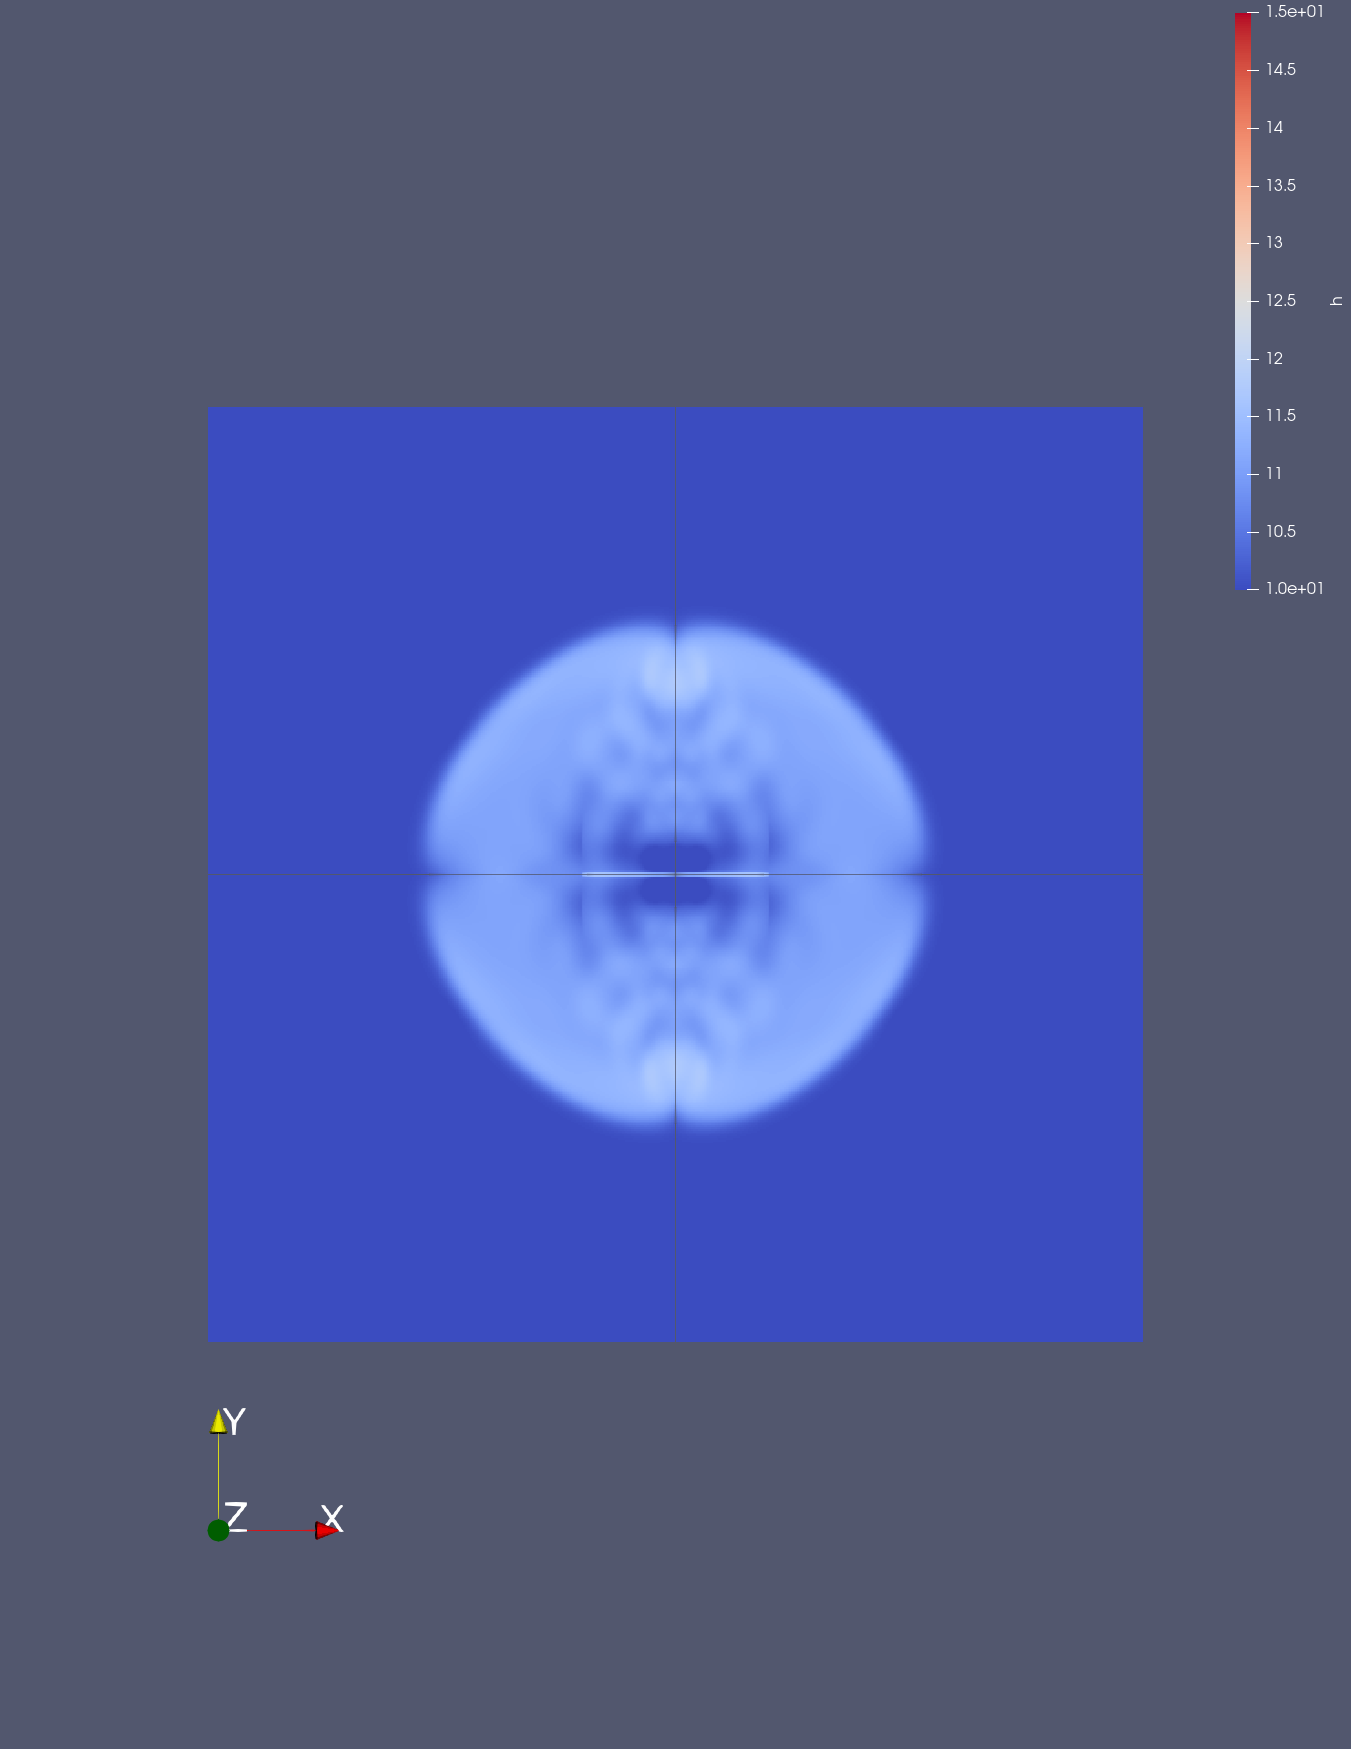
\includegraphics[width=\textwidth,keepaspectratio=true]{figs/1_validation_cuda_original_4mpi.png}
			\caption{4 MPI-CUDA}
			\label{fig:1mpi-cuda-original}
		\end{subfigure}
		%
		%\begin{subfigure}{.2\textwidth}
		%	\centering
		%	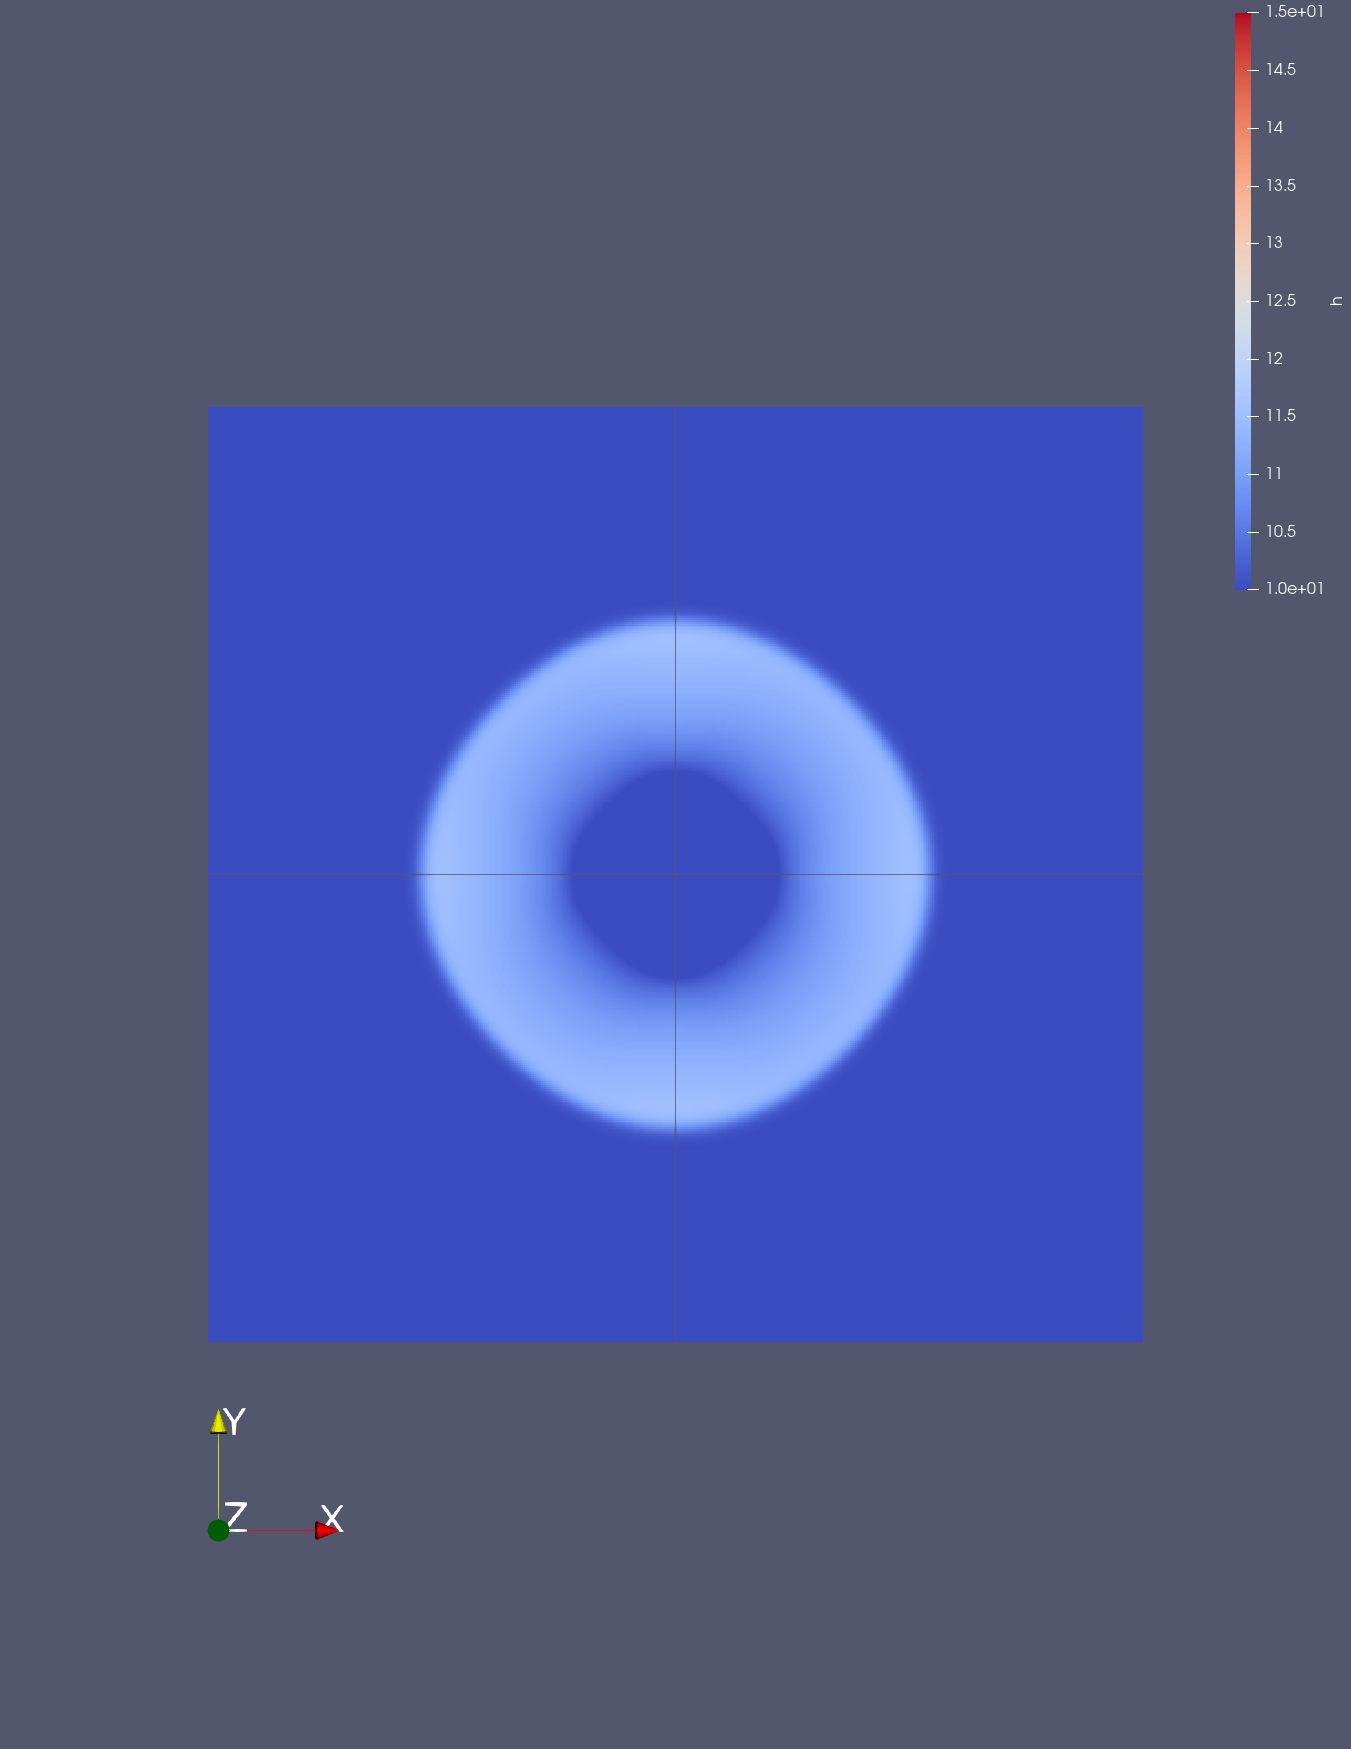
\includegraphics[width=\textwidth,keepaspectratio=true]{figs/1_validation_cuda_fixed_4mpi.png}
		%	\caption{4 MPI-CUDA (after)}
		%	\label{fig:1mpi-cuda-fixed}
		%\end{subfigure}
		\caption{Visualisation of \textit{WaterHeight}}
		%\label{figs:validation_cuda}
	\end{figure}
\end{column}

\begin{column}{0.45\textwidth}
	\vfill
	\vskip4em
\begin{table}

	\begin{tabular}{ |c|c|c|c|}
		\hline
		& 1 cuda      & 4 mpi  & 4 cuda \\
		\hline
		1 mpi & 0.0275     & 0.0373& 29929 \\
		\hline
		1 cuda& 0.0000     & 0.0648& 29929 \\
		\hline
	\end{tabular}
\caption{Abs difference of \textit{h}}
\end{table}
\end{column}
\end{columns}
\end{frame}

\begin{frame}{SWE-CUDA Correction (2)}
\begin{columns}
	\begin{column}{.48\textwidth}
	%	\begin{figure}[htpb]
	%	\centering
	%	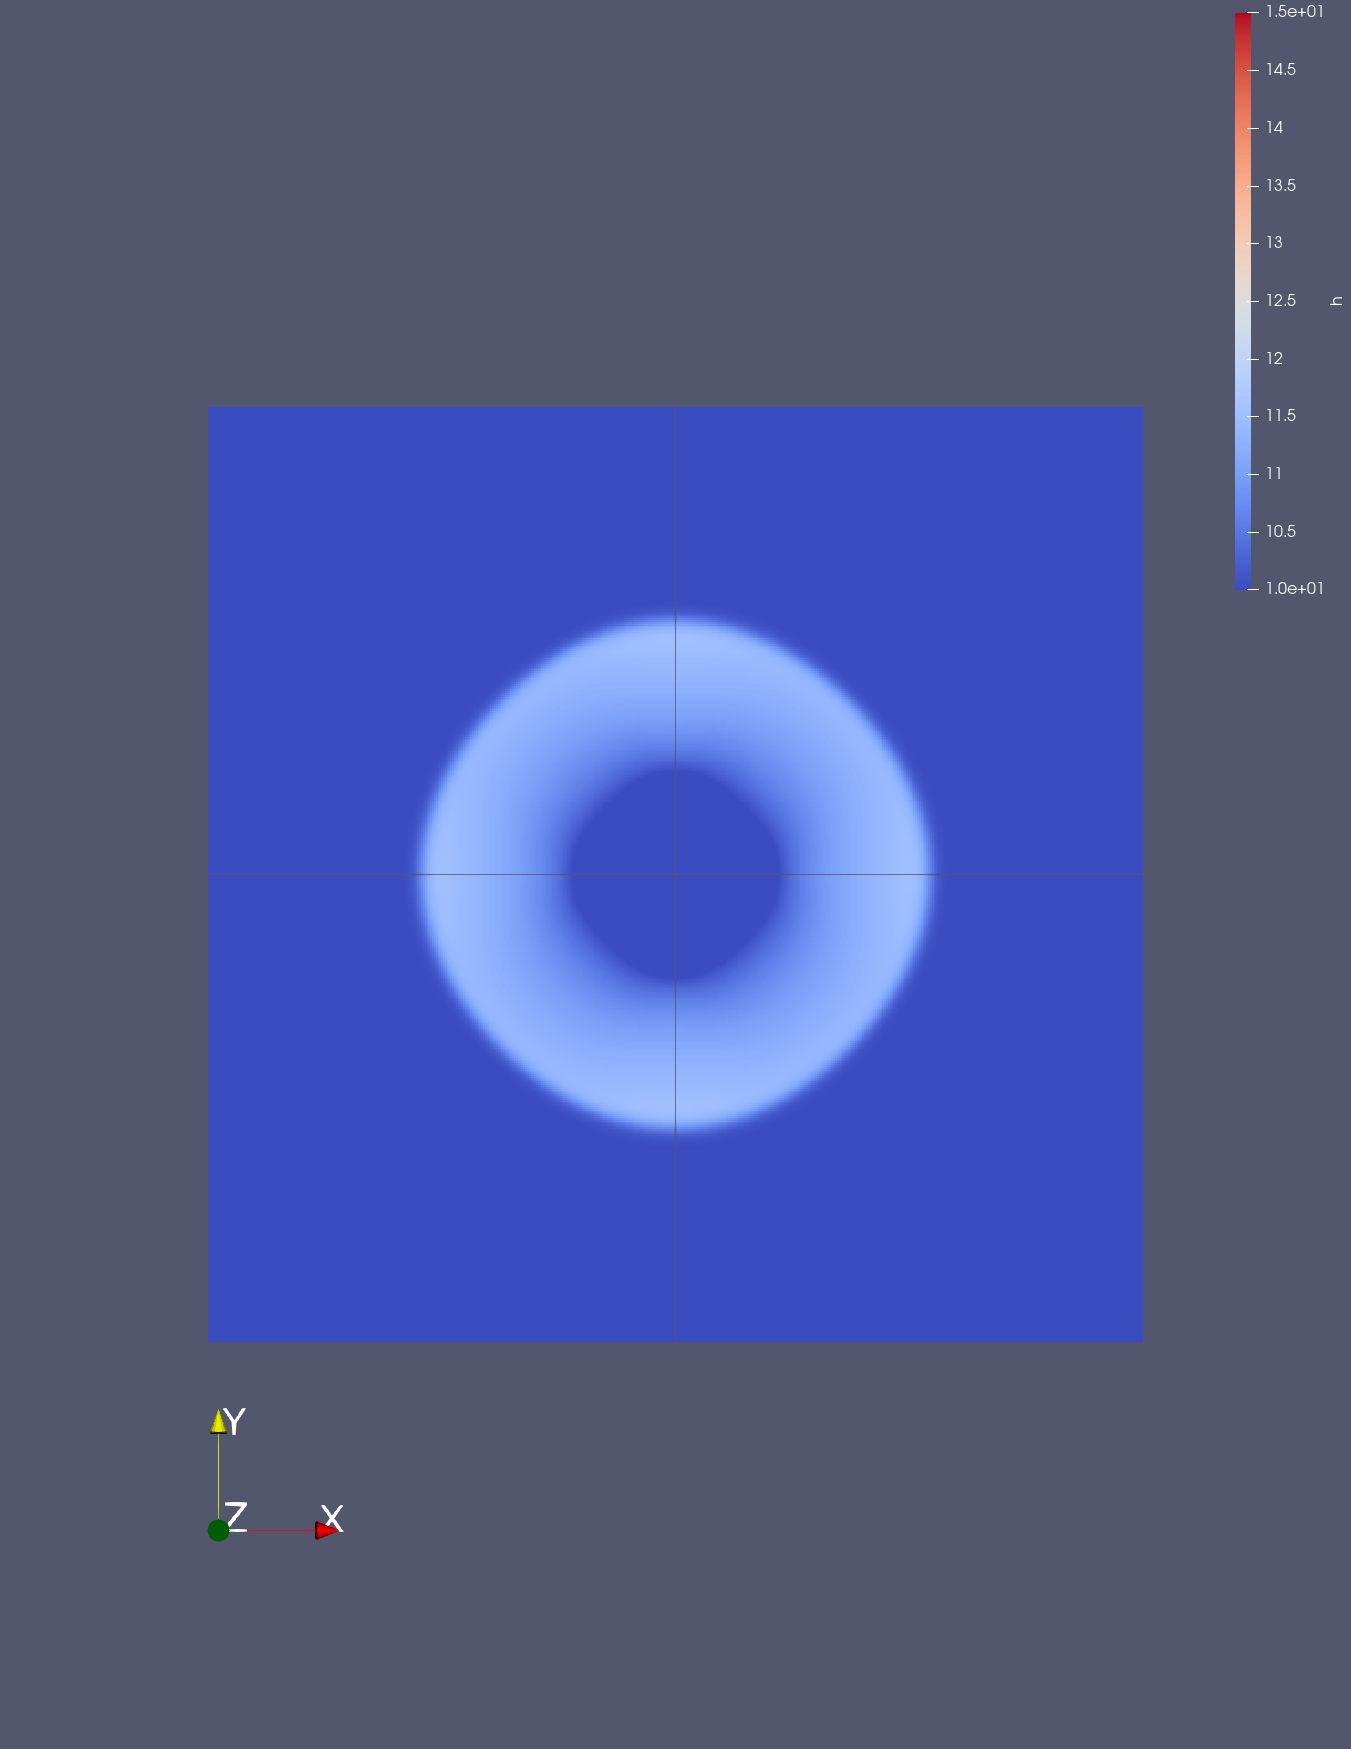
\includegraphics[width=\textwidth,keepaspectratio=true]{figs/1_validation_cuda_fixed_4mpi.png}
	%	\caption{4 MPI-CUDA (after fixed bugs)}
	%	\end{figure}
	\vfill
	\begin{itemize}
		\item \textit{USE\_MPI} was not defined.\\
		$\rightarrow$ No calls \textit{\small synchCopyLayerBeforeRead}.\\
		$\rightarrow$ No \textit{memcpy D->H}
		\newline
		\item No calls \textit{synchGhostLayerAfterWrite} \\
		$\rightarrow$ No \textit{memcpy H->D}
	\end{itemize}
	\end{column}
	
	\begin{column}{.45\textwidth}
\begin{table}

\begin{tabular}{ |c|c|c|c|}
	\hline
	& 1 cuda      & 4 mpi  & 4 cuda \\
	\hline
	1 mpi & 0.02754     & 1.28397& 0.02754 \\
	\hline
	1 cuda& 0.00000     & 1.31151& 0.00000\\
	\hline
\end{tabular}
\caption{Abs difference of \textit{h} after fixing bugs}	
\end{table}
	\end{column}
\end{columns}
\end{frame}




%%%%%%%%%%%%%%%%%%%%%%%%%%%%%%%%%%%%%%%%%%%%%%%%%%%%%%%%%%%%%%%%%%%%%%%%%%%%%%%
\section{Results and Discussion}
\subsection{Validation}
\begin{frame}[fragile]{Validation}
Runs job on multiple GPUs with the \textit{run\_gpu.sh} script
\begin{columns}
	\begin{column}{.45\textwidth}
\begin{lstlisting}[frame=single] 
#!/bin/bash
export CUDA_VISIBLE_DEVICES=\
	$OMPI_COMM_WORLD_LOCAL_RANK
case $OMPI_COMM_WORLD_LOCAL_RANK in
[0]) cpus=0;;
[1]) cpus=1;;
[2]) cpus=2;;
[3]) cpus=3;;
esac
numactl --physcpubind=$cpus $@
\end{lstlisting}
%The command to run the simulation with multiple GPUs is as follow:
\begin{lstlisting}
$ mpirun -np 4 ../gpu_bind.sh ./swe-cuda 
		-x ${NX} -y ${NY} -c ${STEPS} -o .
\end{lstlisting}
	\end{column}

	\begin{column}{0.45\textwidth}
		\begin{figure}[htpb]
			\centering
			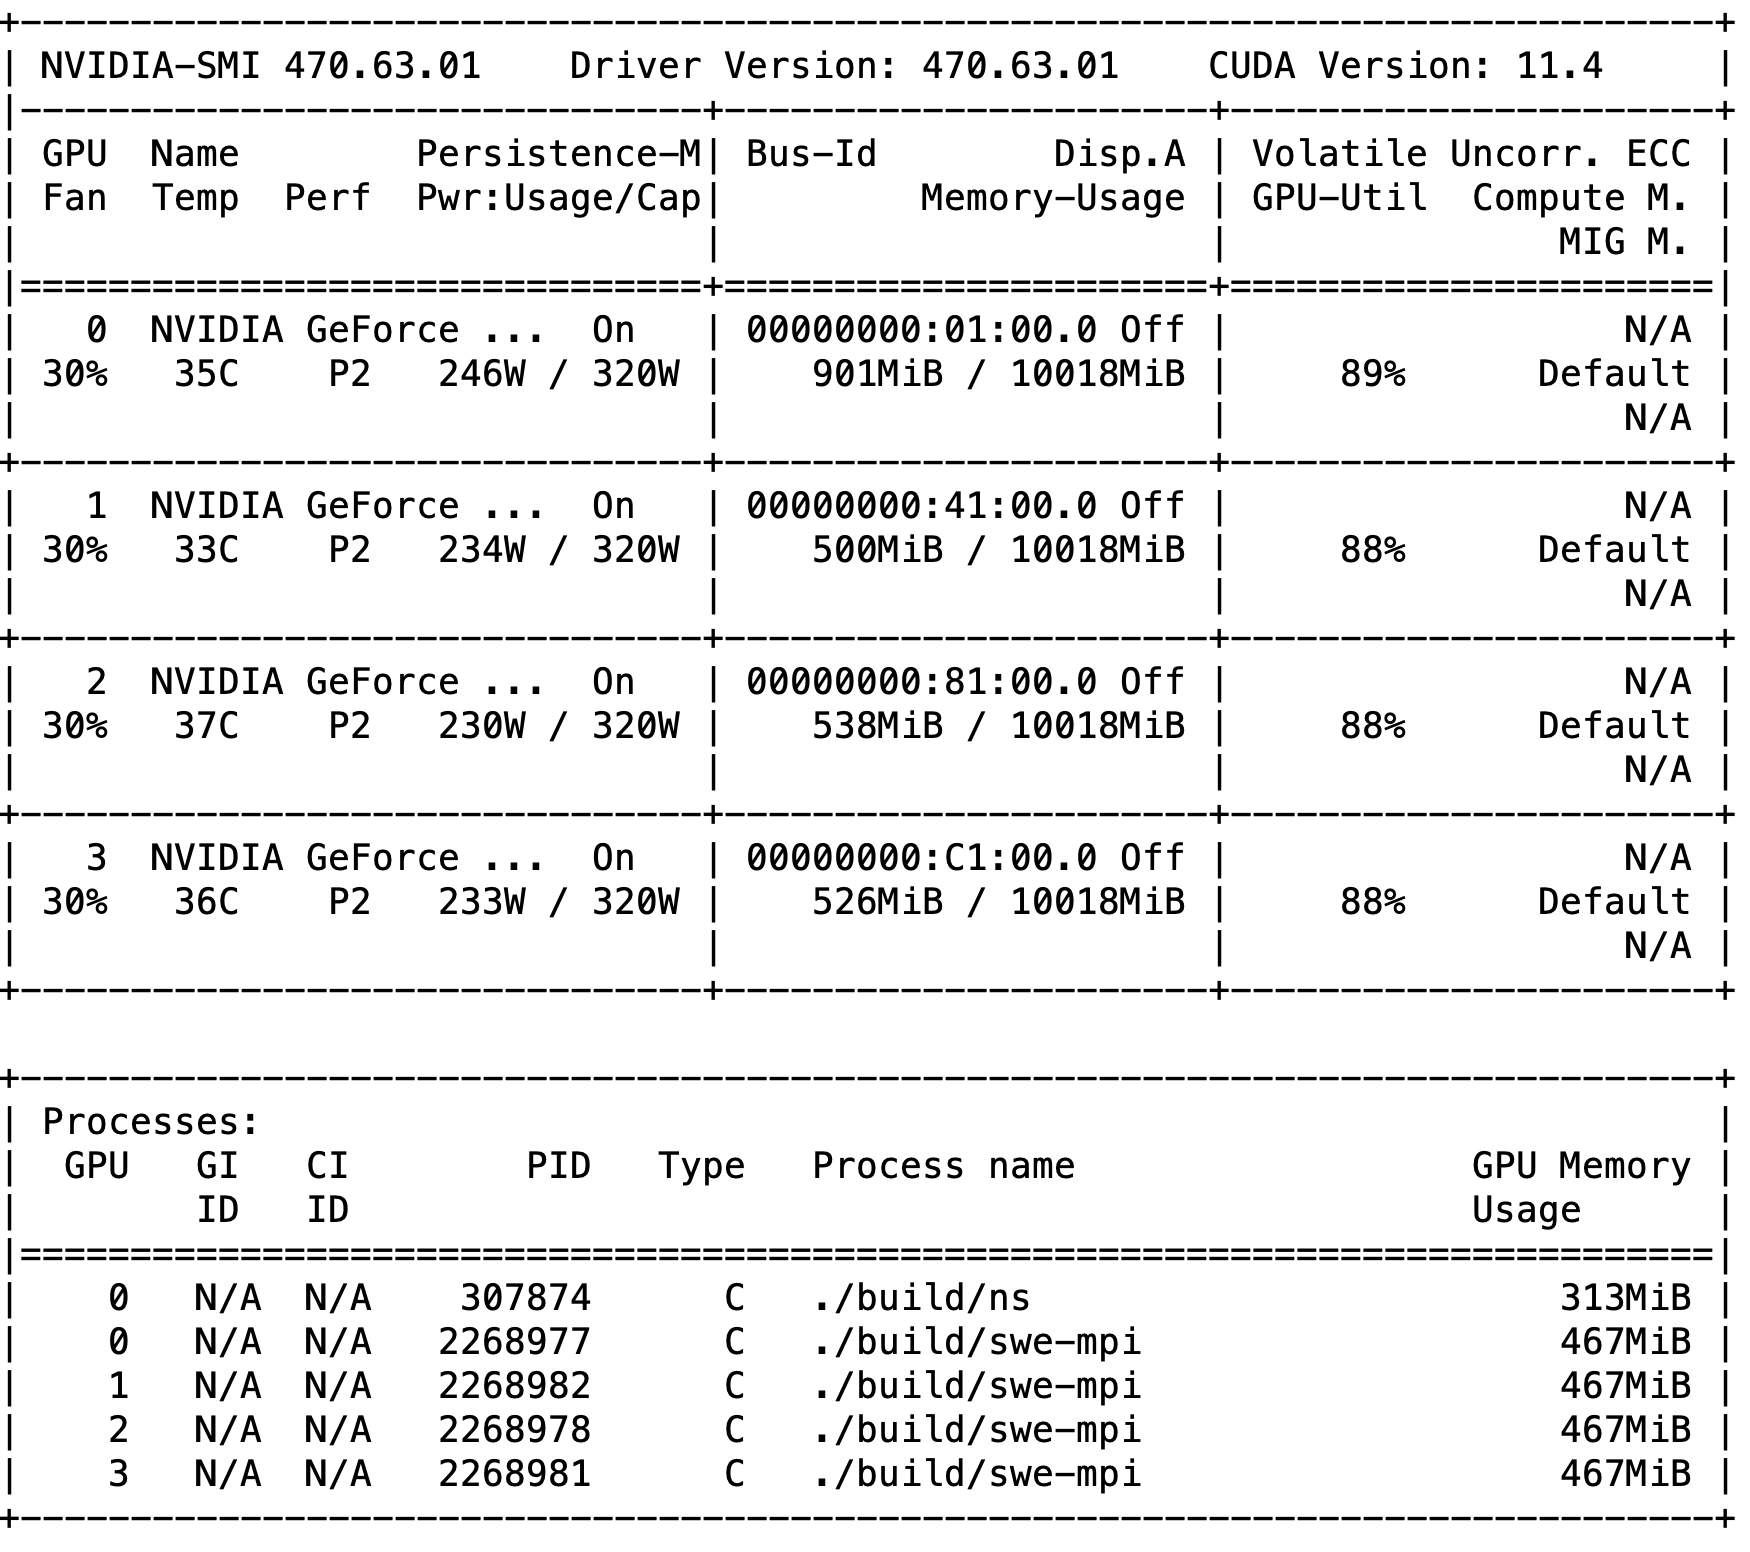
\includegraphics[width=0.9\textwidth,keepaspectratio=true]{figs/cuda4096-4.png}
			\caption{GPU Monitoring}
			\label{fig:GPUMonitor}
		\end{figure}
	\end{column}
\end{columns}

\end{frame}

%--------------------------------------------------------------------
\begin{frame}{Validation}
\begin{columns}
	\begin{column}{.45\textwidth}
		 \begin{figure}[htpb]
			\centering
			\begin{subfigure}{.48\textwidth}
				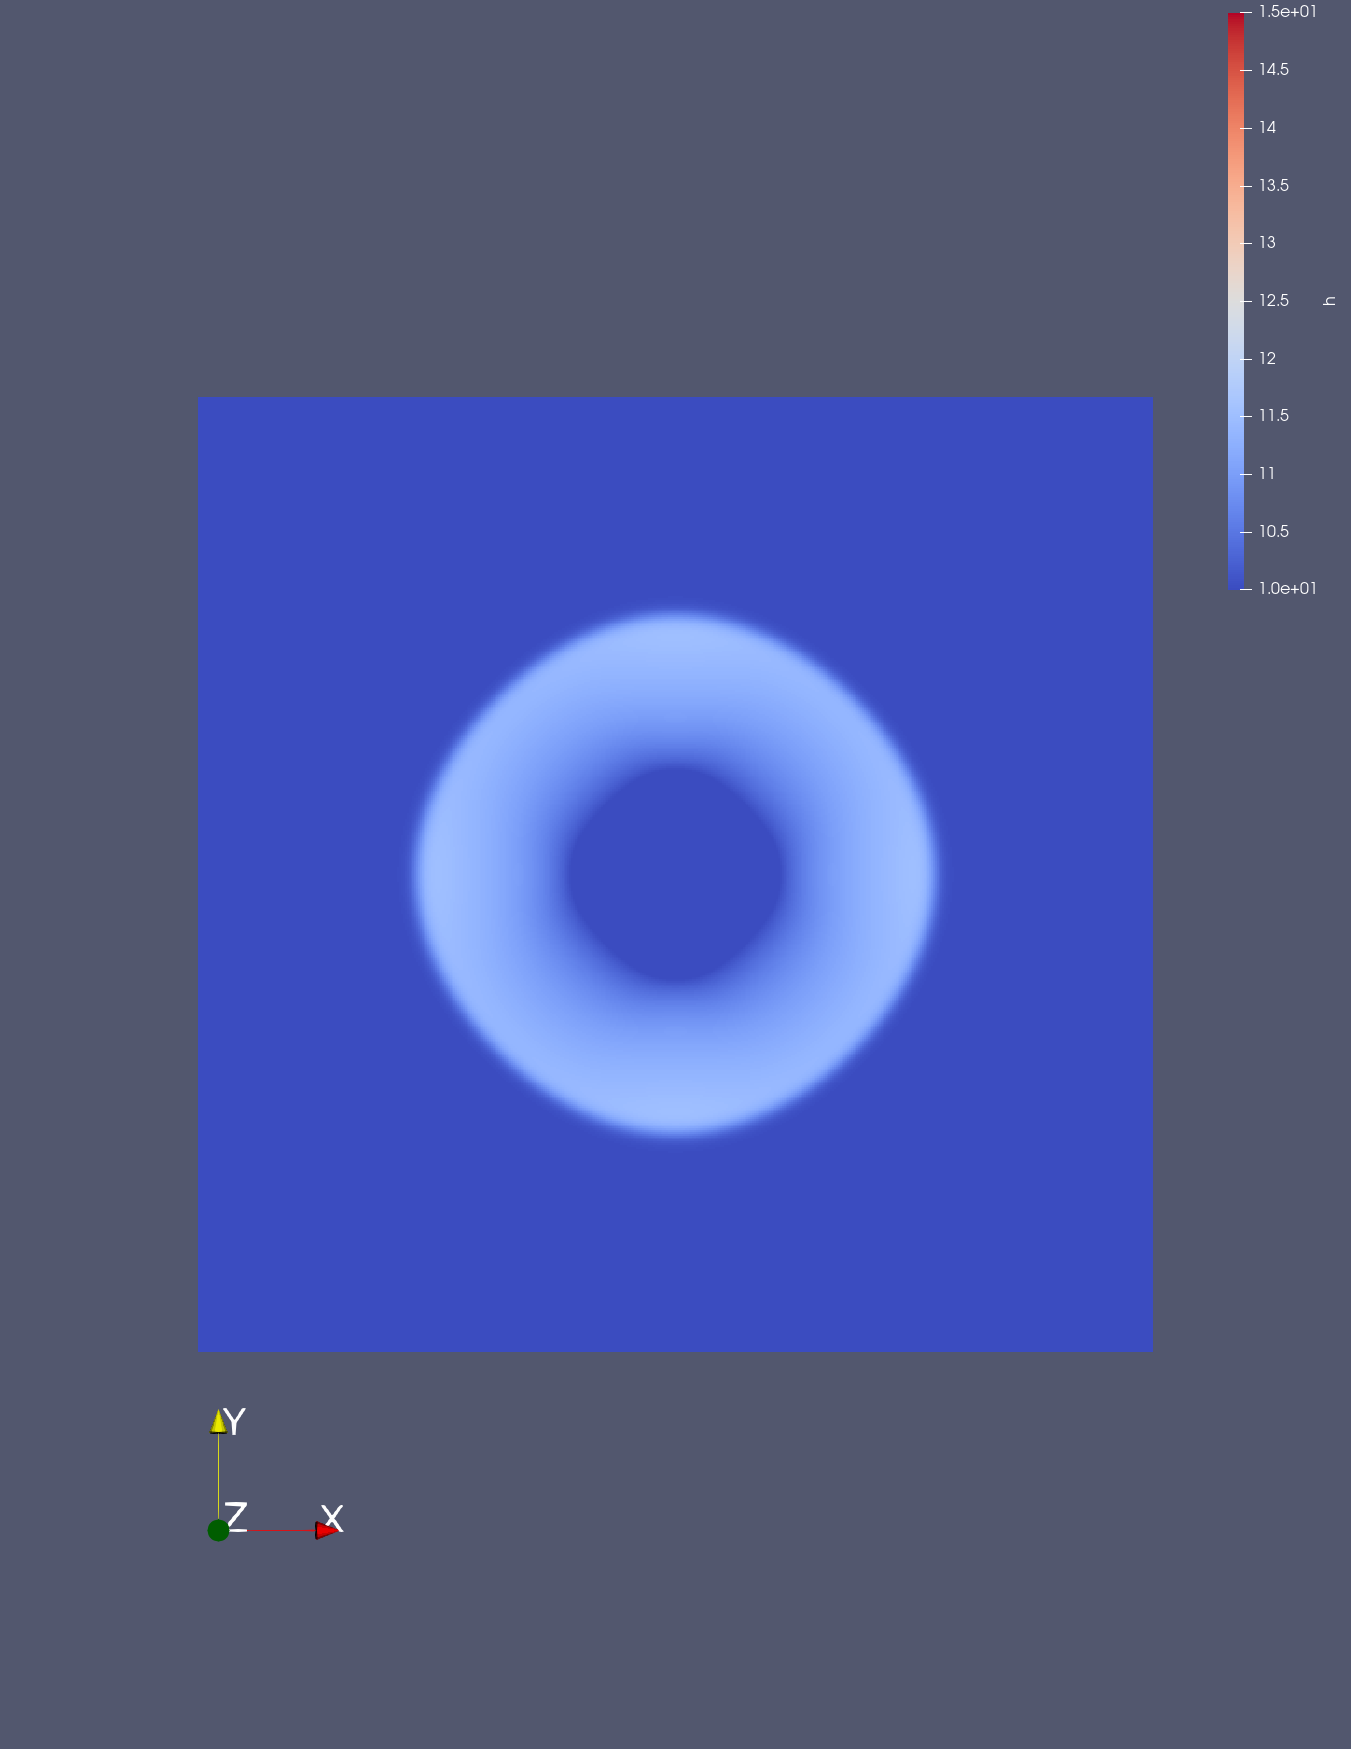
\includegraphics[width=\textwidth,keepaspectratio=true]{figs/1_validation_cuda_original_1mpi.png}
				%   \caption{1 MPI (no CUDA)}
				\label{fig:1mpi_2nd}
			\end{subfigure}
			%
			\begin{subfigure}{.48\textwidth}
				\centering
				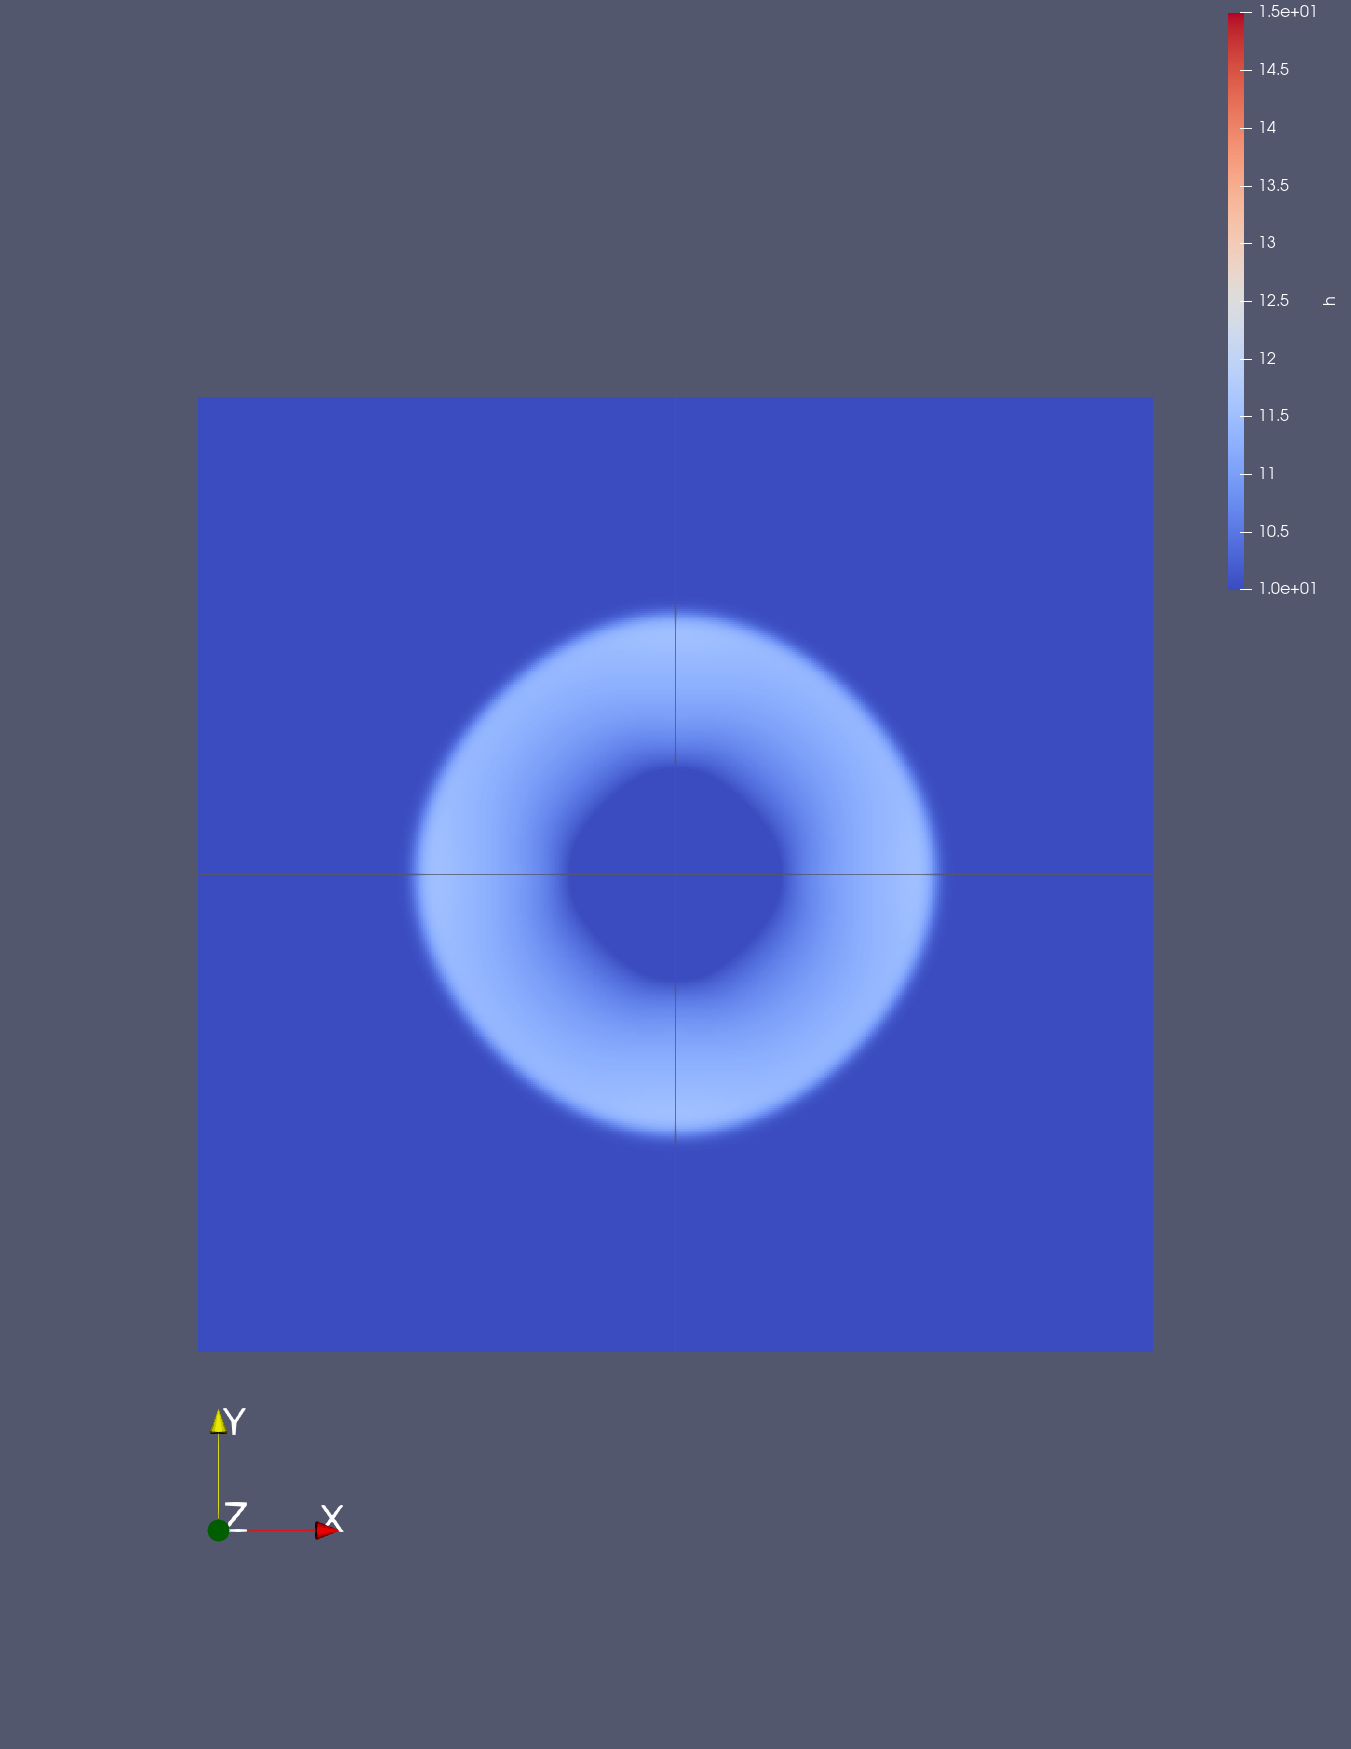
\includegraphics[width=\textwidth,keepaspectratio=true]{figs/1_validation_cuda_aware_4mpi.png}
				%\caption{4 CUDA-Aware-MPI)}
				\label{fig:4mpi-cuda-aware}
			\end{subfigure}
			\caption{Pure-MPI vs CUDA-Aware-MPI}
			\label{figs:validation_cuda_aware}
		\end{figure}
	\end{column}
	\begin{column}{.4\textwidth}
		CUDA-Aware MPI implementation produced correct results.
		\begin{table}[h!]
			\centering
			\begin{tabular}{ |c|c|c|}
				\hline
				& 1 cuda-aware& 4 cuda-aware \\
				\hline
				1 mpi & 0.0275     & 0.0275 \\
				\hline
				1 cuda& 0.0000     &  0.0000 \\
				\hline
				4 cuda& 0.0000     & 0.0000 \\
				\hline
			\end{tabular}
			\caption{Error table}
			\label{table:cuda_aware}
		\end{table}  
	\end{column}
\end{columns}

\end{frame}
%-----------------------------------------------------------
\subsection{Initial Performance}
\begin{frame}{Initial Performance}
\begin{figure}[htpb]
	\centering
	\begin{subfigure}{.45\textwidth}
		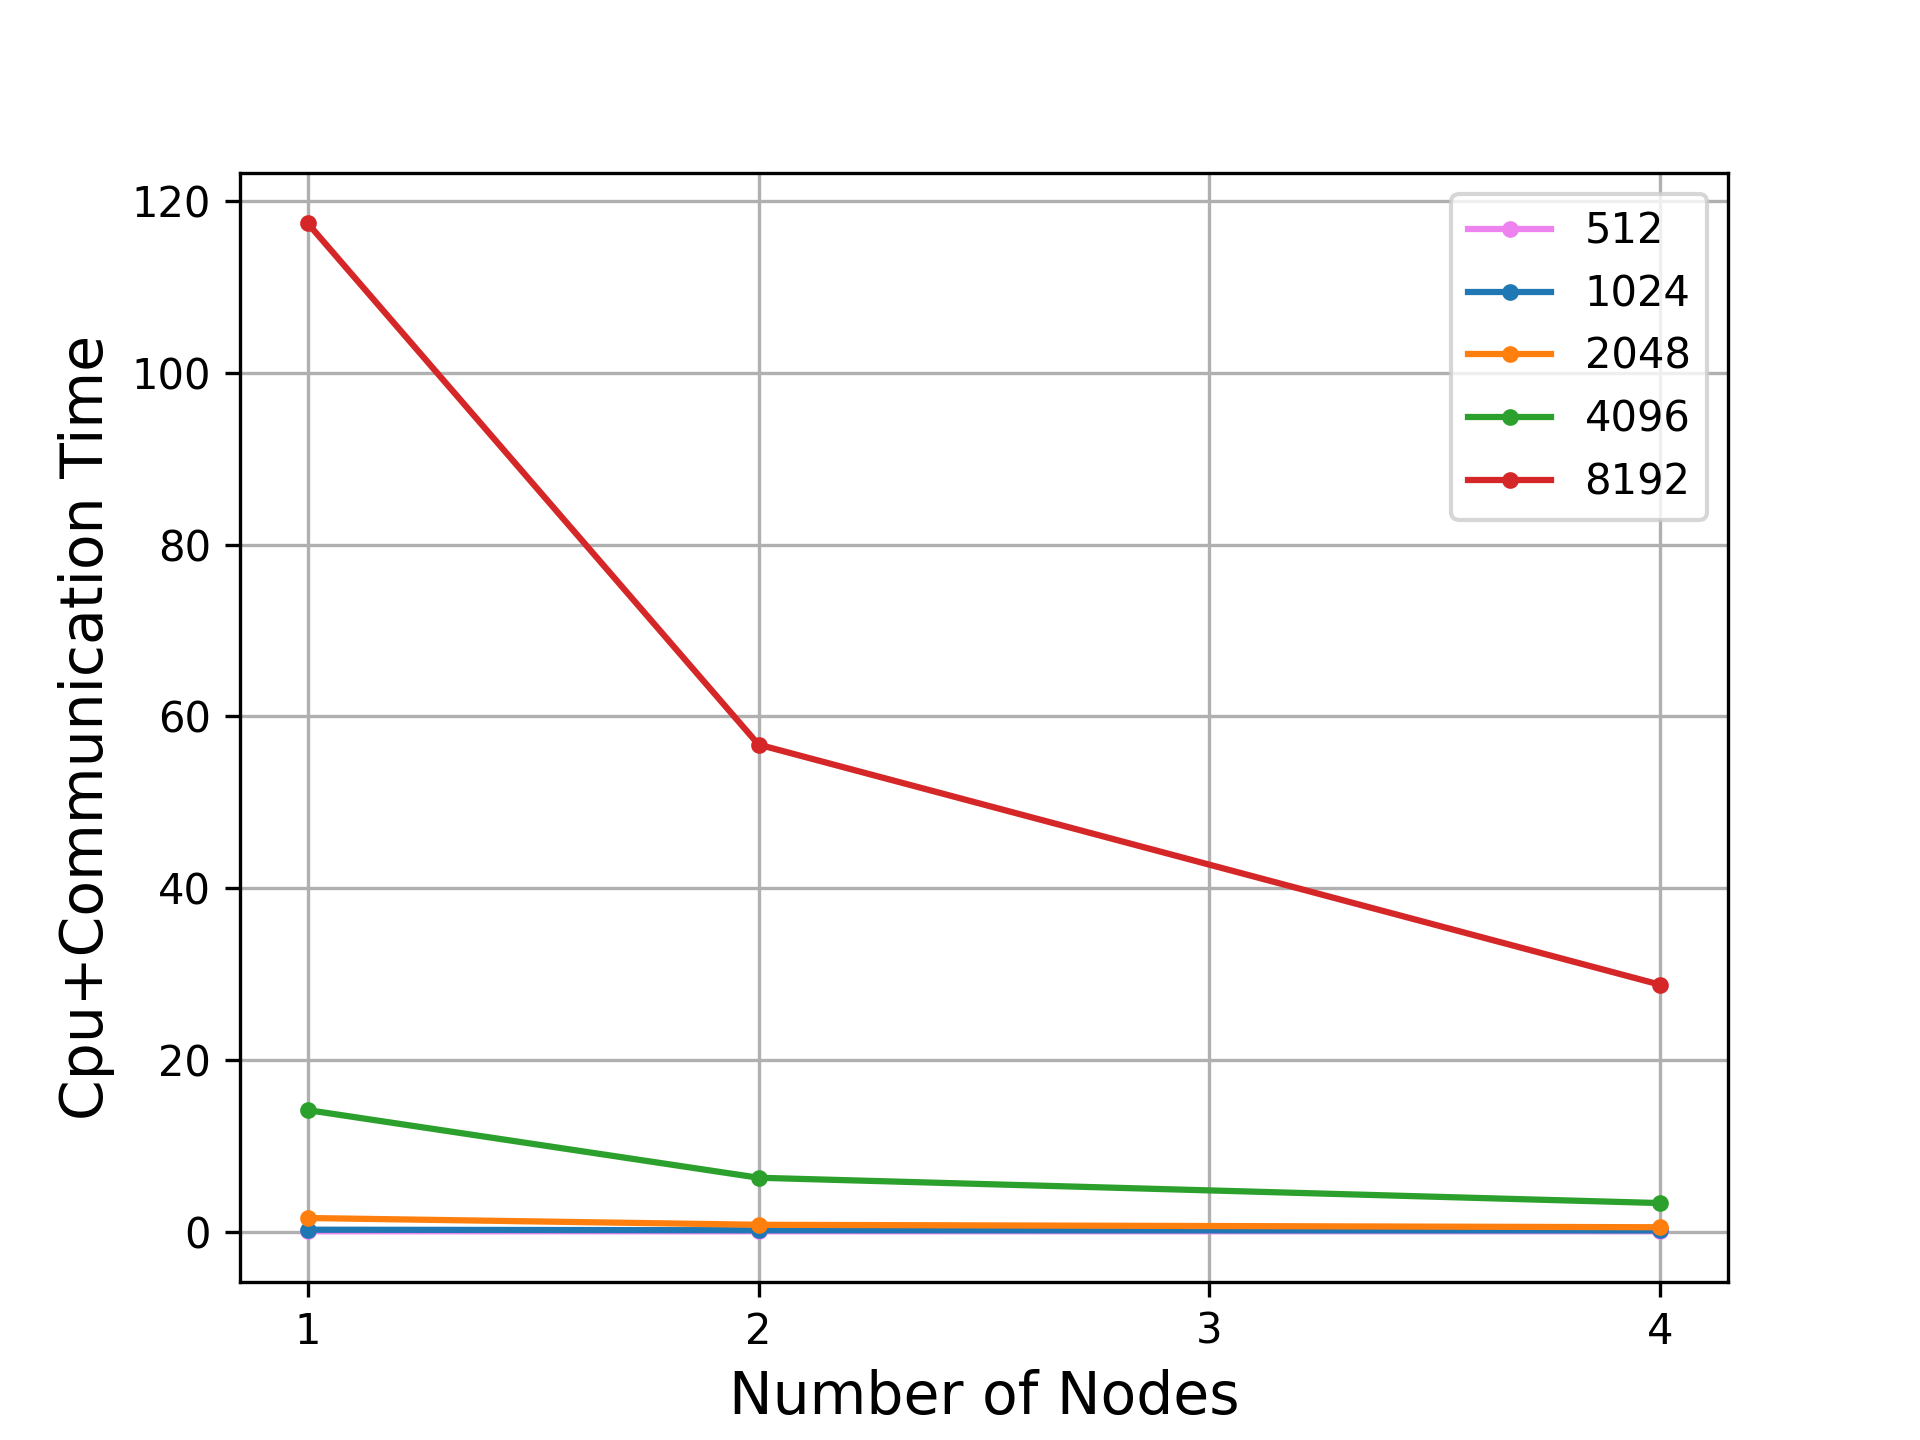
\includegraphics[width=\textwidth,keepaspectratio=true]{figs/strongscalingCOMM_CUDA.png}
		\caption{normal CUDA+MPI}
		\label{fig:StrongCOMMCUDA}
	\end{subfigure}
	%
	\begin{subfigure}{.45\textwidth}
		\centering
		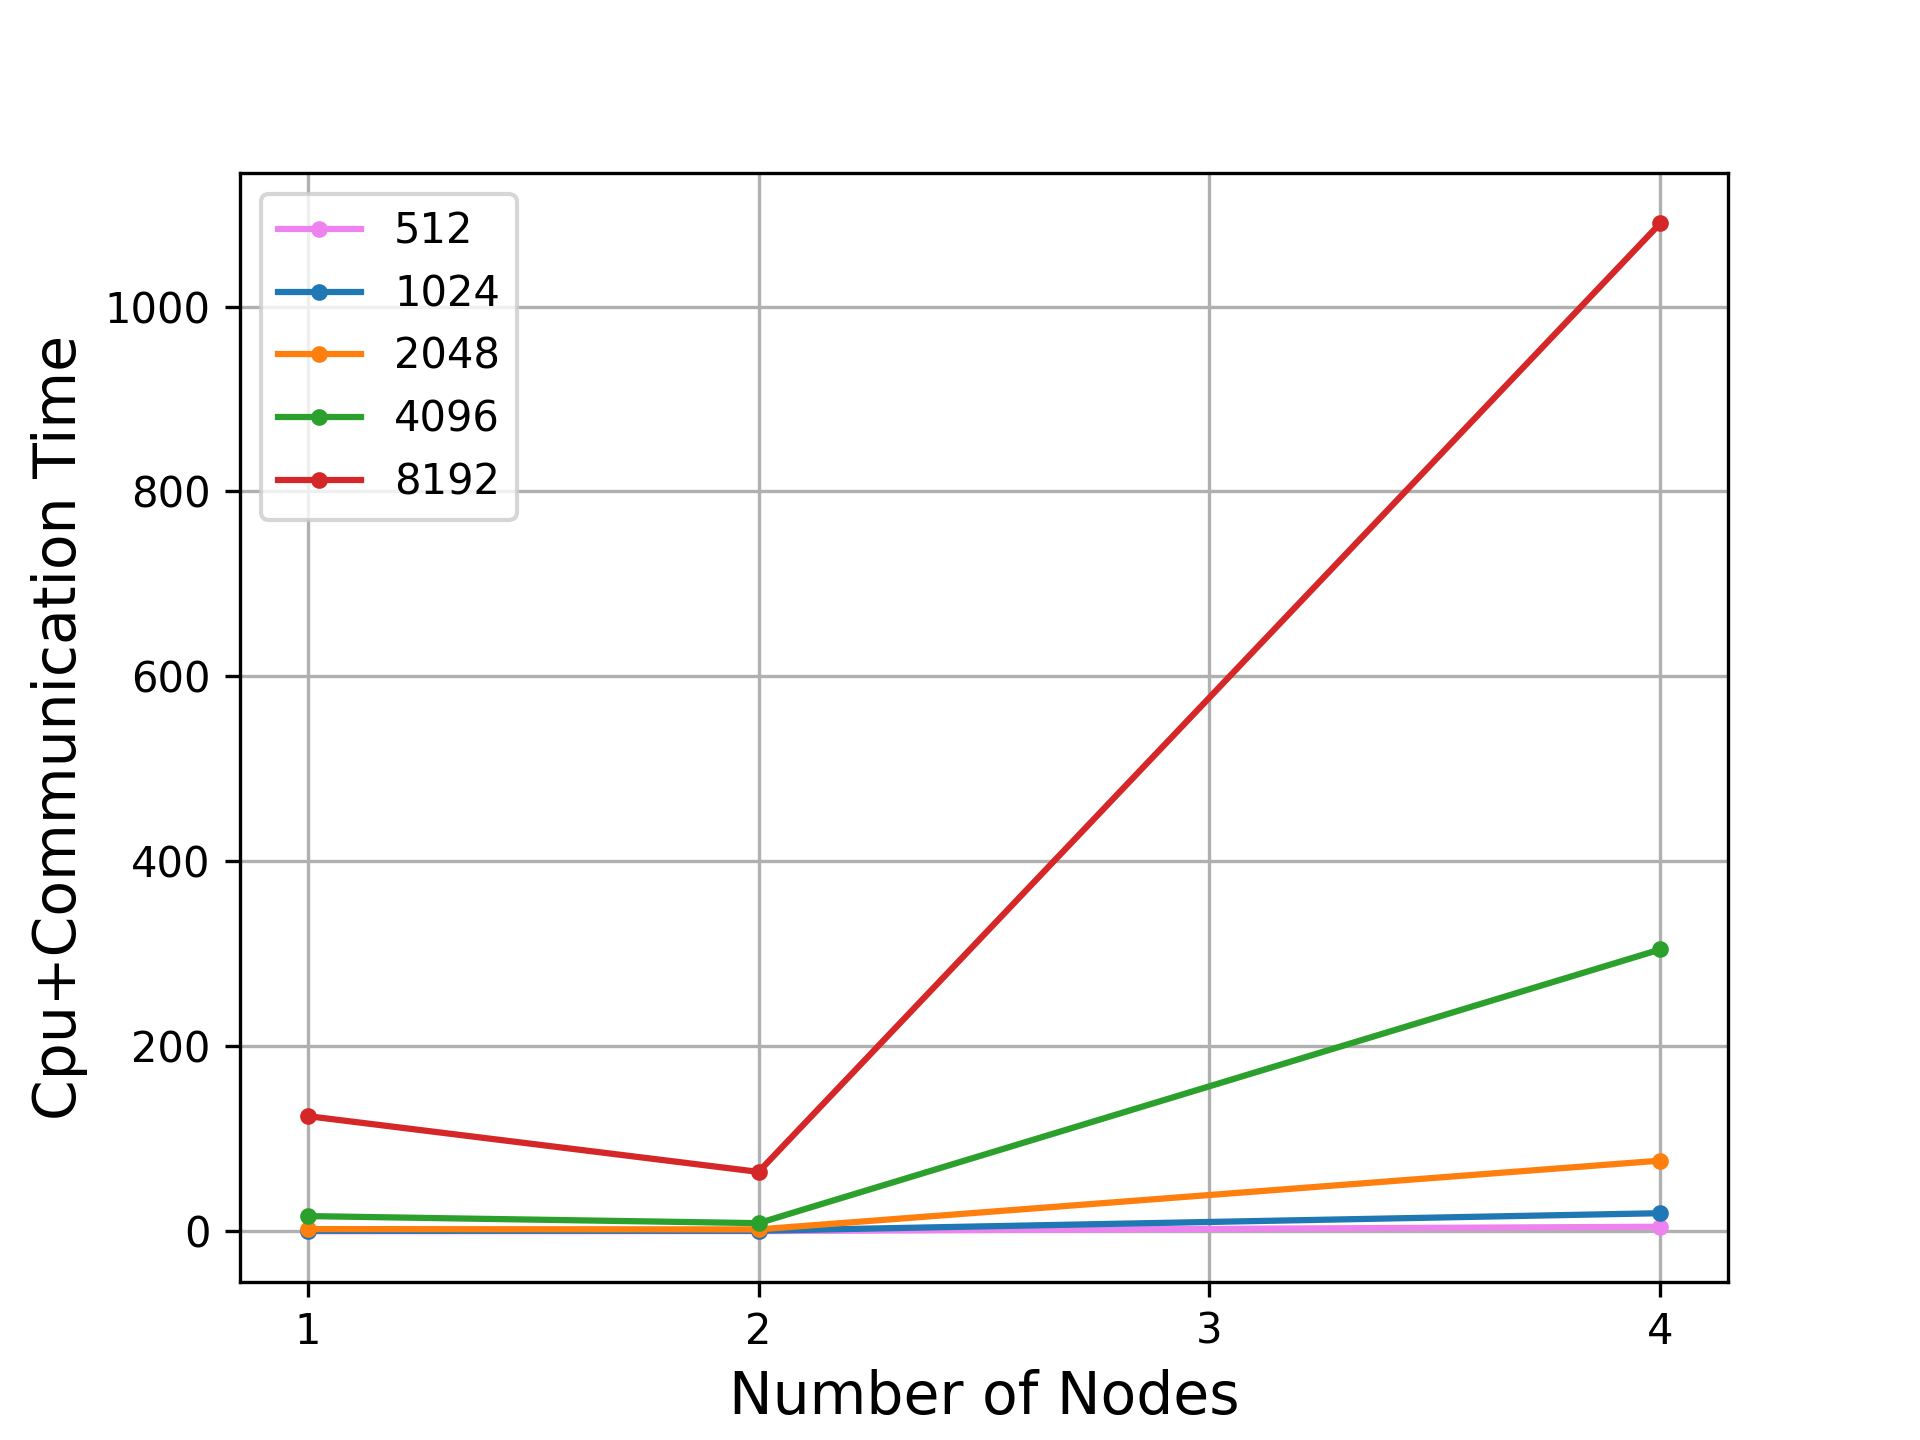
\includegraphics[width=\textwidth,keepaspectratio=true]{figs/strongscalingCOMM.png}
		\caption{CUDA-Aware-MPI}
		\label{fig:StrongCOMM}
	\end{subfigure}
	\caption{Runtime comparison of the two implementations}
	\label{figs:Compare2}
\end{figure}
\end{frame}
% ---------------------------------------------
\begin{frame}{Hardware specs}
\begin{columns}
	\begin{column}{.36\textwidth}
		\vskip3em
		\textbf{NVIDIA GeForce RTX™ 3080 ?} \\
		$\rightarrow$ No NVLINK \\
		$\rightarrow$ No GPUDirect support \\
	\end{column}
	\begin{column}{.5\textwidth}
			\vskip-2em
\begin{figure}
	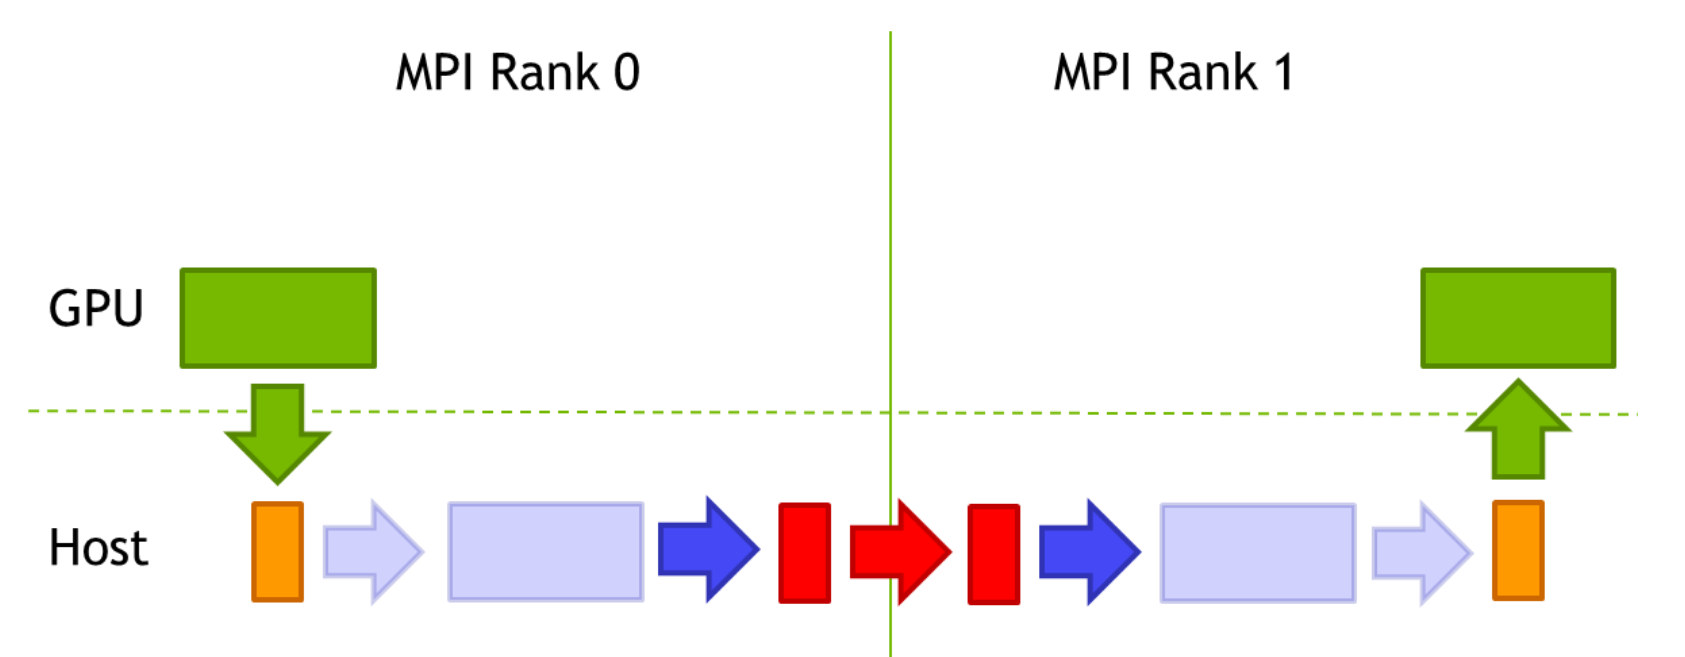
\includegraphics[width=\textwidth,keepaspectratio=true]{figs/nogpudirect1.png}
\end{figure}
	\vskip-2em
\begin{figure}
	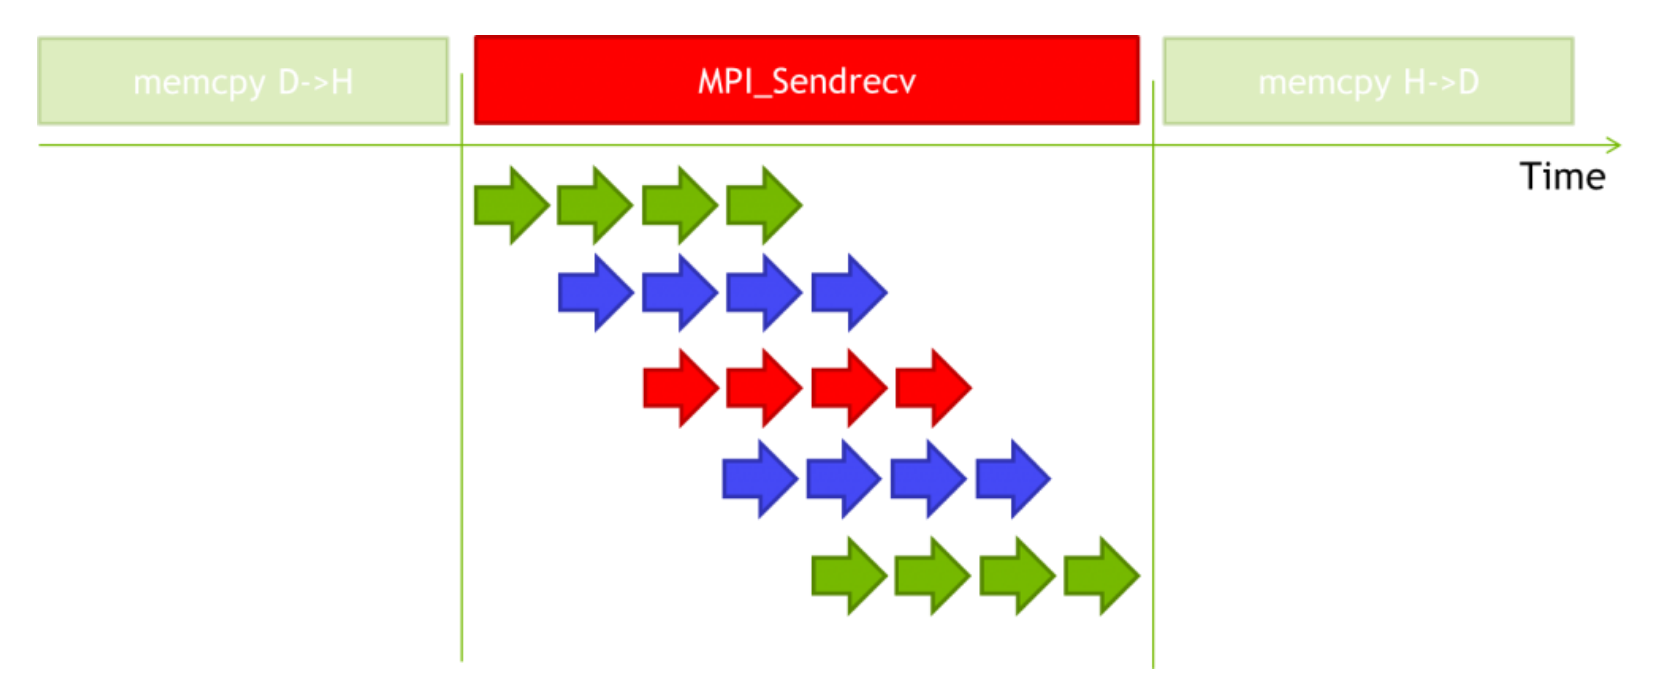
\includegraphics[width=\textwidth,keepaspectratio=true]{figs/nogpudirect2.png}
	\vskip5em
	\caption{CUDA-Aware MPI 222}
\end{figure}		
	\end{column}
\end{columns}
	
	
	
\end{frame}


%---------------------------------------------------------
\begin{frame}[fragile]{Profiling Output}
\begin{columns}
	\begin{column}{.48\textwidth}
\tiny
\begin{lstlisting}[frame=single,language=C++,caption={2 MPI}, captionpos=b]
Time(%)  Time (ms)     Name    
------- ---------  ---------------------
   76.4       292  cudaMallocManaged    
   13.9        53  cudaDeviceSynchronize
    4.8        18  cudaLaunchKernel    
    1.7         6  cudaMemcpyAsync  
      
Time(%)  Time (ms)     Operation    
-------  --------  ---------------------
   47.1      2  [CUDA Unified Memory memcpy HtoD]
   39.4      2  [CUDA Unified Memory memcpy DtoH]
   13.5      1  [CUDA memcpy DtoH] 
     

Time(%)  Time (ms)        Range
-------  --------  ---------------------
   44.8       171  MPI:MPI_Init
   28.8       110  MPI:MPI_Finalize
   15.4        58  MPI:MPI_Sendrecv
   11.0        42  MPI:MPI_Allreduce
\end{lstlisting}		
	\end{column}
	\begin{column}{.48\textwidth}
\tiny
\begin{lstlisting}[frame=single,language=C++,caption={4 MPI}, captionpos=b]
Time(%)  Time (ns)     Name    
-------  --------  ---------------------
   62.7      3342  cuMemcpyAsync    
   26.2       139  cuStreamSynchronize  
    9.4       499  cudaMallocManaged    
    1.1        57  cudaDeviceSynchronize
    
Time(%)  Time (ns)     Operation
-------  --------  ---------------------
   52.6    527  [CUDA memcpy HtoD]
   46.6    467  [CUDA memcpy DtoH]
    0.4      4  [CUDA Unified Memory memcpy HtoD]
    0.3      3  [CUDA Unified Memory memcpy DtoH]
    
Time(%)  Time (ns)        Range
-------  --------  ---------------------
   92.4      7147  MPI:MPI_Sendrecv
    3.7       288  MPI:MPI_Init
    2.4       187  MPI:MPI_Allreduce
    1.5       115  MPI:MPI_Finalize
\end{lstlisting}	
	\end{column}
\end{columns}


\end{frame}

%%%%%%%%%%%%%%%%%%%%%%%%%%%%%%%%%%%%%%%%%%%%%%%%%%%%%%%%%%%%%%%%%%%%%%%%%%%%%%%

\section{Optimization}

\begin{frame}[fragile]{Data Packing}
\begin{columns}
	\begin{column}{.46\textwidth}
%\vskip1em
\tiny
\begin{lstlisting}[frame=single,language=c++, captionpos=b, label={profile3}]
l_waveBlock->setGhostLayer();
while (iteration) // time integration loop
{
exchangeGhostLayers();

synchGhostLayerAfterWrite(); //data unpacking;
l_waveBlock->computeNumericalFluxes();

MPI_Allreduce(&maxTimeStep, &maxTimeGlobal,...);

l_waveBlock->updateUnknowns(l_maxTimeGlobal);
synchCopyLayerBeforeRead() // data packing

iteration++;
}
\end{lstlisting}
	\end{column}
	\begin{column}{.45\textwidth}
		\vskip-2em
		\begin{figure}[htpb]
			\centering
			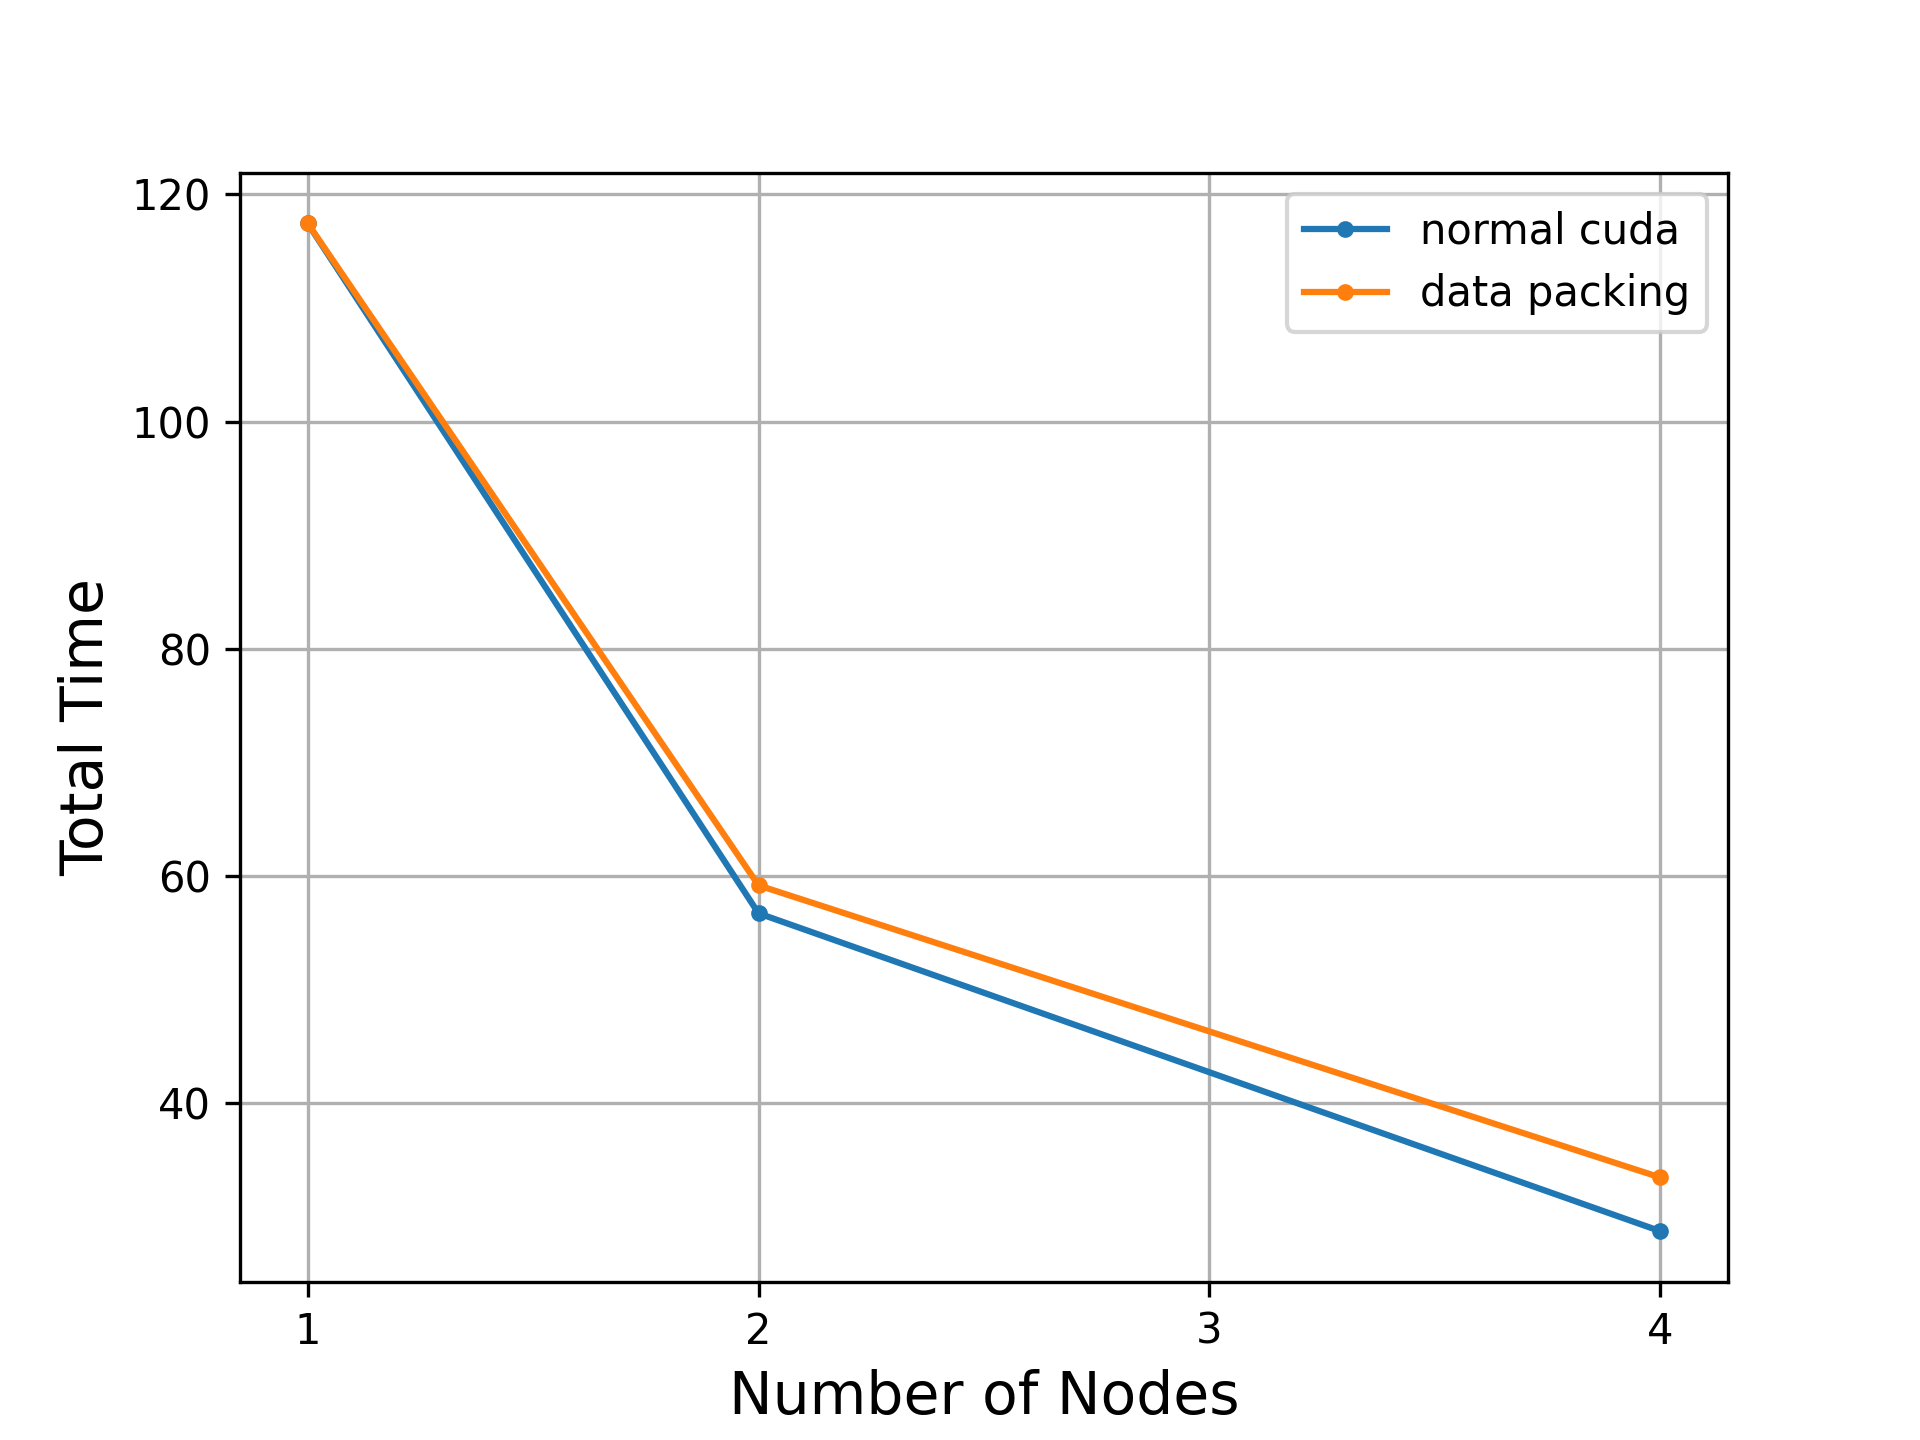
\includegraphics[width=\textwidth,keepaspectratio=true]{figs/Comparison_CUDA_PACKING.png}
		\caption{Performance improvement with Packing}
		\end{figure}

	\end{column}
\end{columns}
    
\end{frame}
%%%%%%%%%%%%%%%%%%%%%%%%%%%%%%%%%%%%%%%%%%%%%%%%%%%%%%%%%%%%%%%%%%%%%%%%%%%%%%%

\begin{frame}{Data Migration}
\begin{columns}
	\begin{column}{.50\textwidth}
		\vskip3em
	\begin{itemize}
		\item \textit{cudaMemAdvise}
		\begin{itemize}
			\item \textit{cudaMemAdviseSetPreferredLocation}
			\item \textit{cudaMemAdviseSetAccessedBy}
		\end{itemize}
		\item \textit{cudaMemPrefetchAsync}
	\end{itemize}	
	\end{column}
	\begin{column}{.48\textwidth}
		\vskip-2em
	\begin{figure}[htpb]
		\centering
		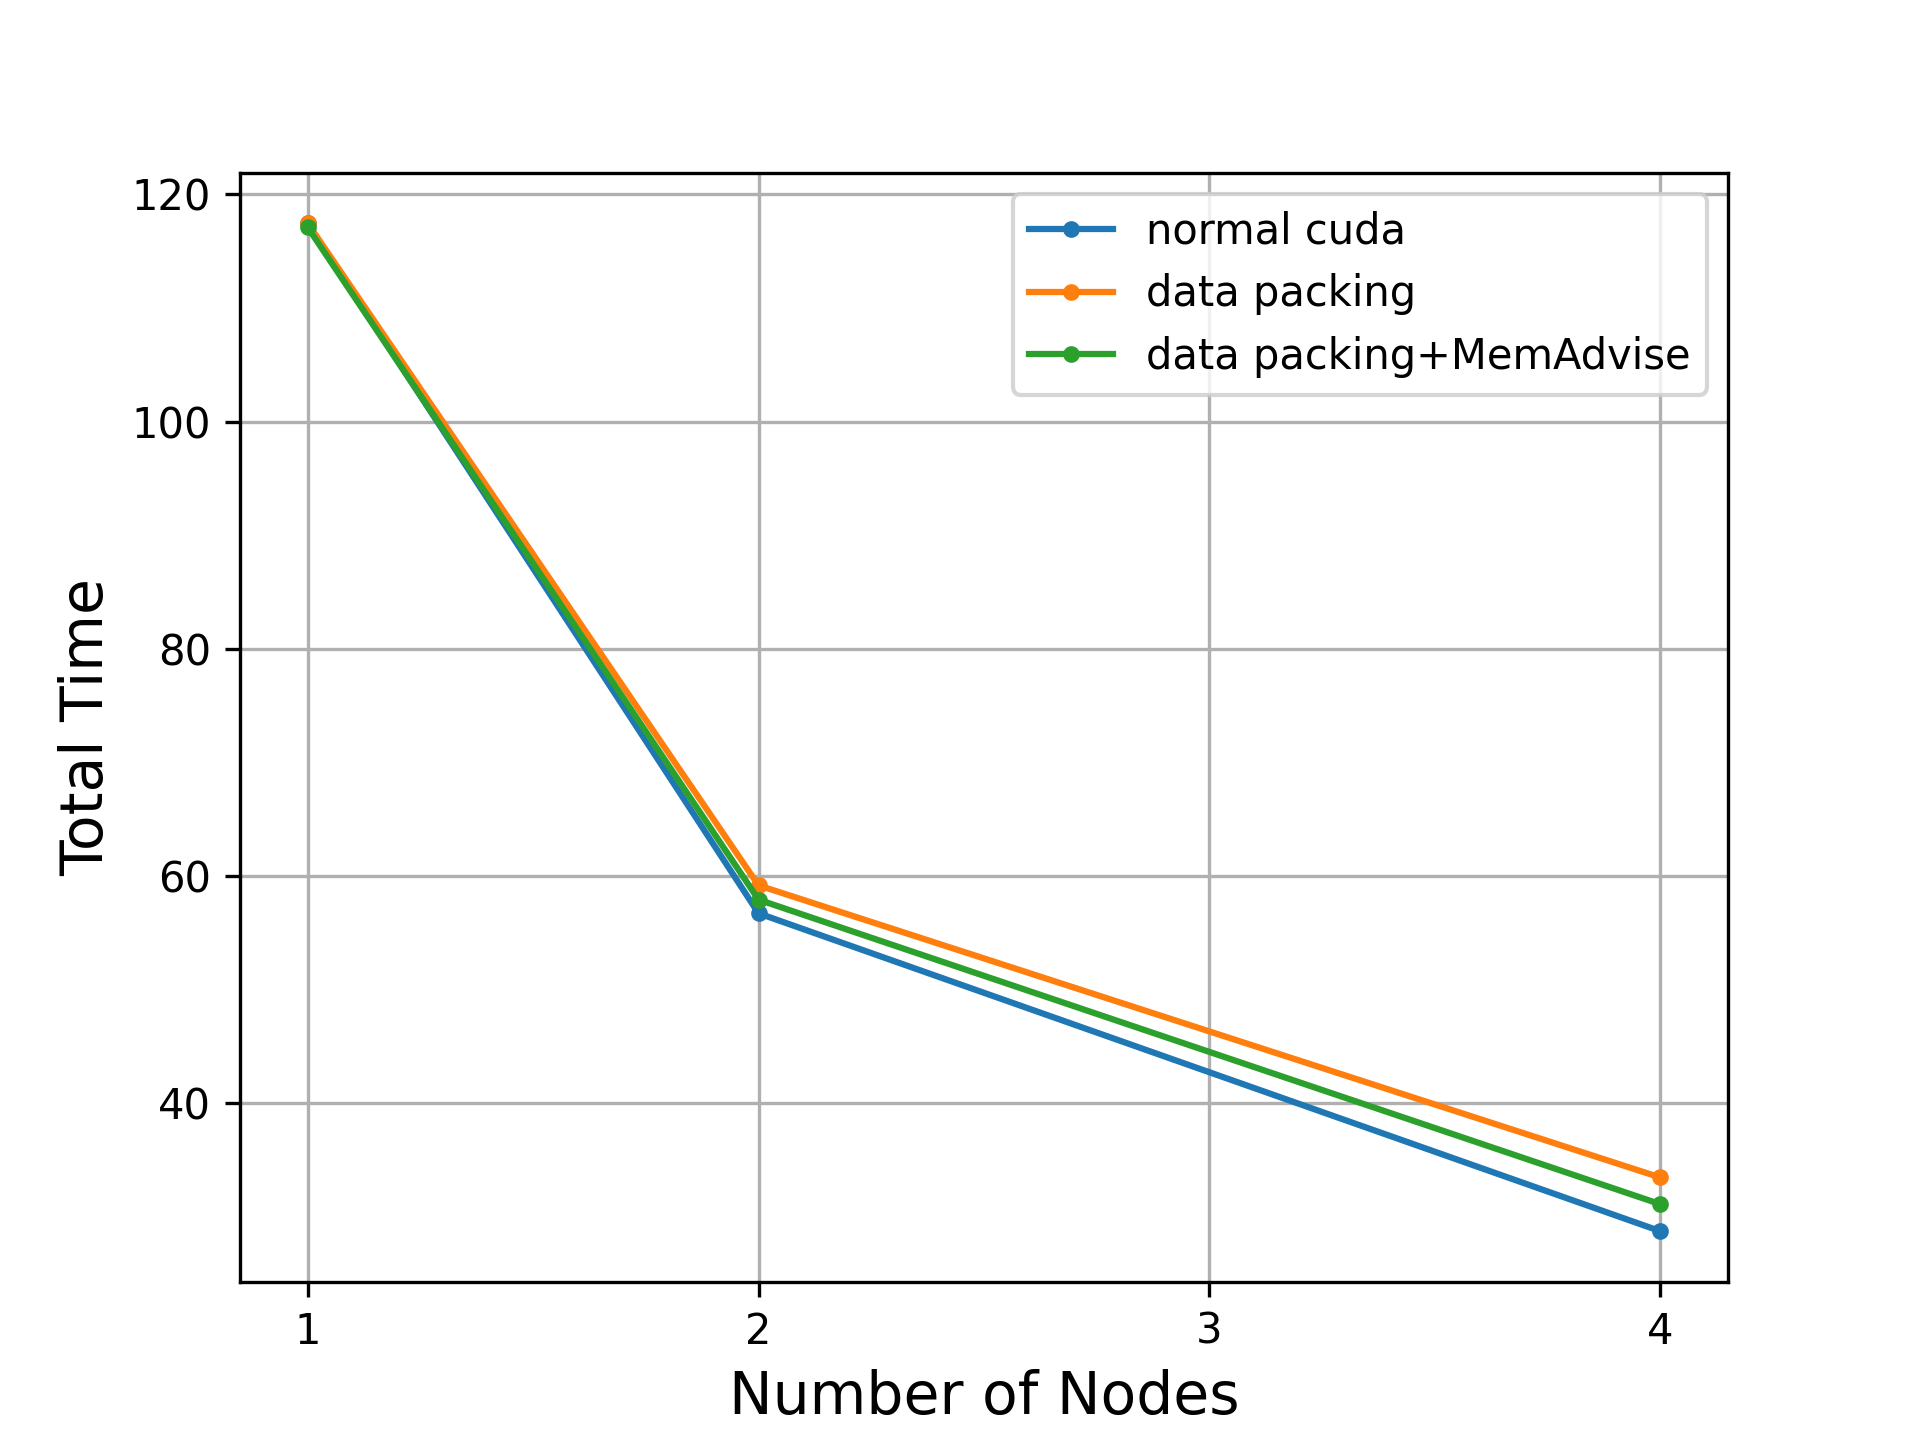
\includegraphics[width=\textwidth, keepaspectratio=true]{figs/Comparison_CUDA_PACKING_MemAdvise.png}
		\caption{Performance improvement with MemAdvise}
	\end{figure}
	\end{column}
\end{columns}

\end{frame}



%%%%%%%%%%%%%%%%%%%%%%%%%%%%%%%%%%%%%%%%%%%%%%%%%%%%%%%%%%%%%%%%%%%%%%%%%%%%%%%

\begin{frame}{Non Blocking Communication}
	\begin{columns}
		\begin{column}{.50\textwidth}
			\vskip3em
\begin{itemize}
	\item \textit{MPI\_Isend} and \textit{MPI\_Irecv}
	\item Only communication overlap, no overlap with computations
\end{itemize}
		\end{column}
		\begin{column}{.48\textwidth}
			\vskip-2em
   \begin{figure}[htpb]
	\centering
	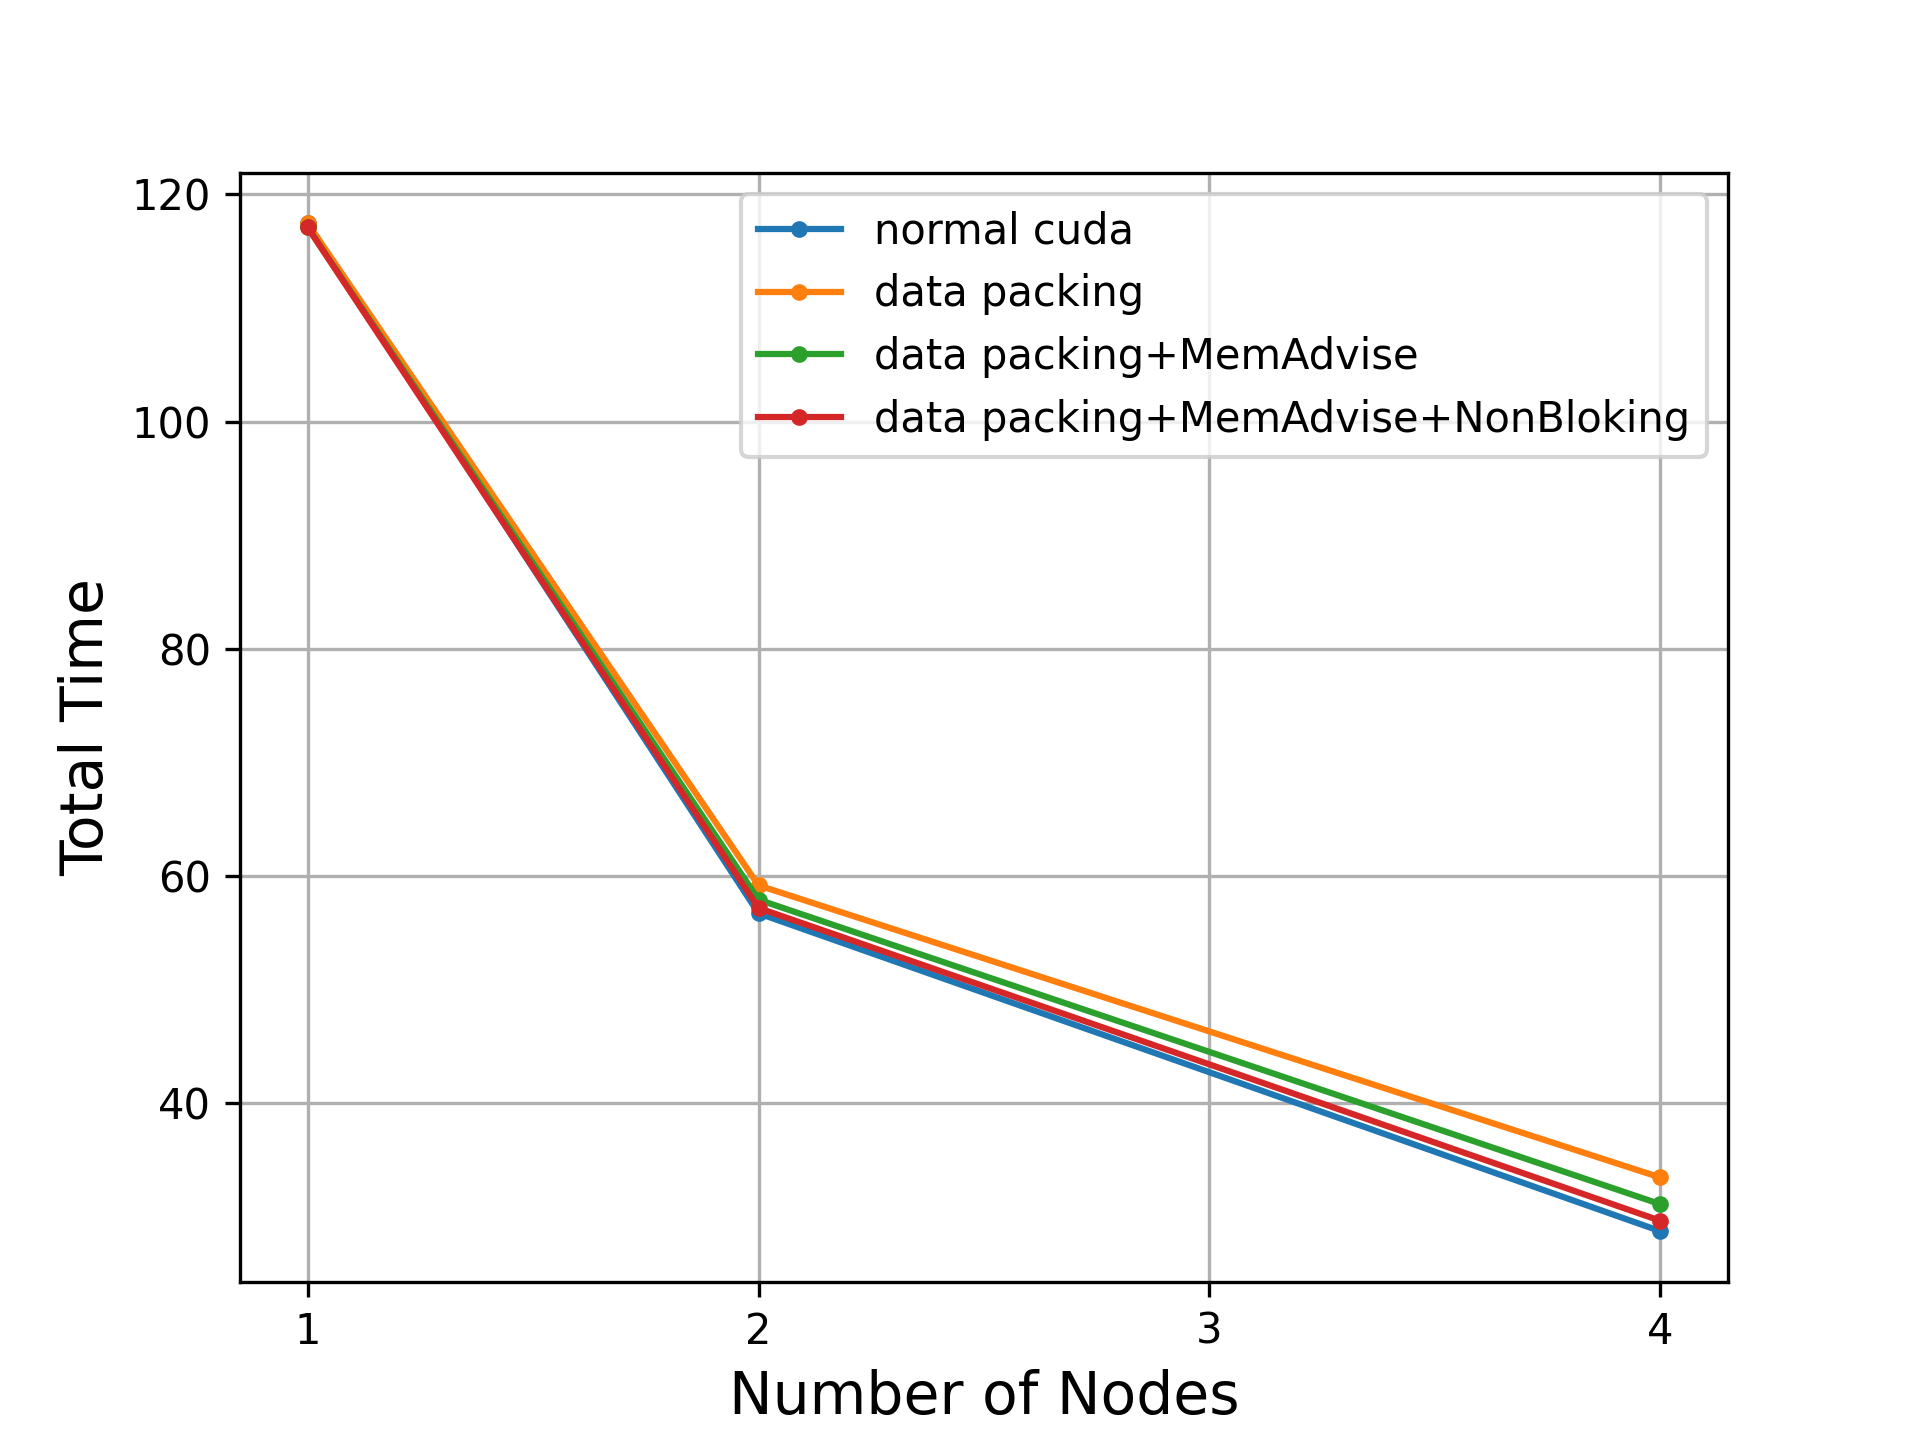
\includegraphics[width=\textwidth, keepaspectratio=true]{figs/Comparison_CUDA_PACKING_MemAdvise_NonBlocking.png}
	\caption{Performance improvement with Non Blocking}
\end{figure}
		\end{column}
	\end{columns}
  
    \end{frame}


%%%%%%%%%%%%%%%%%%%%%%%%%%%%%%%%%%%%%%%%%%%%%%%%%%%%%%%%%%%%%%%%%%%%%%%%%%%%%%%
\section{Future Work \& Conclusion}

\begin{frame}{Future Work}
			\vfill
	\begin{columns}
		\begin{column}{.8\textwidth}
			\begin{itemize}
				\item Testing the implementation with different Runtime optimization: \\
				GPU Direct RMDA, GPU Direct P2P, MPS, etc
				\newline
				\item Overlapping Computations with Communications.
			\end{itemize}
		\end{column}
	\end{columns}
	\vfill	
   
\end{frame}



%%%%%%%%%%%%%%%%%%%%%%%%%%%%%%%%%%%%%%%%%%%%%%%%%%%%%%%%%%%%%%%%%%%%%%%%%%%%%%%


\begin{frame}[fragile]{Conclusion}
	\vskip1em
    \begin{columns}
        \begin{column}[t]{0.45\textwidth}
            \begin{itemize}
                \item Successfully implemented CUDA-Aware MPI for SWE
                \item Fixed some bugs of the original code
                \item Achieved almost the same performance as the normal cuda version using CUDA-Aware-MPI without GPUDiect support
            \end{itemize}
        \end{column}
        %
        % \begin{minipage}[t]{0.04\textwidth}
        % \end{minipage}
        %
        \begin{minipage}[t]{0.45\textwidth}
        %\fontsize{2}{1}
        \begin{figure}
            %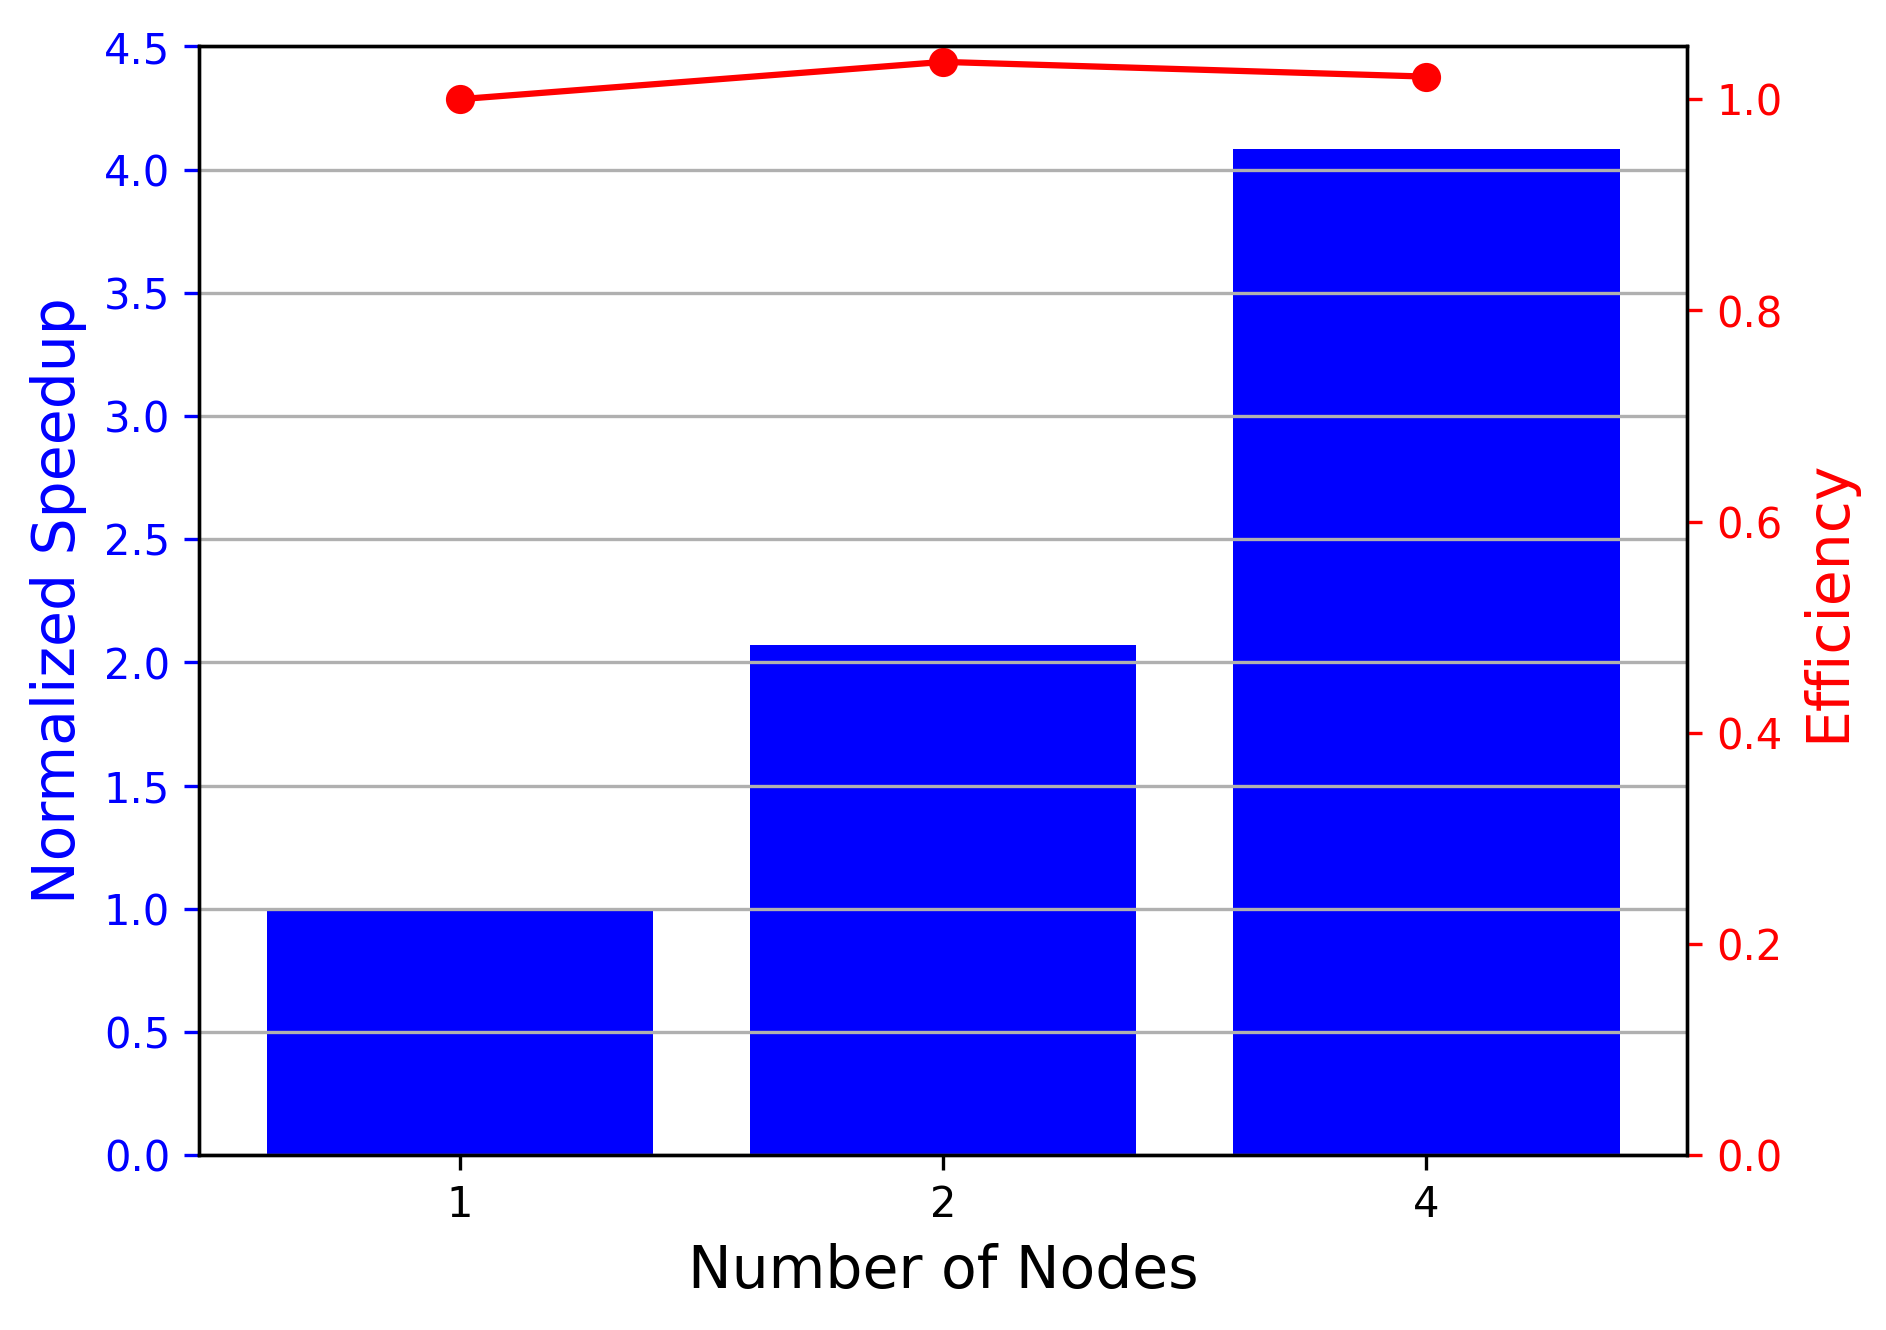
\includegraphics[width=.7\textwidth, height=.4\textheight]{figs/SpeedUp_Eff_COMM_CUDA.png}\\
            %\vspace{0.2cm} 
            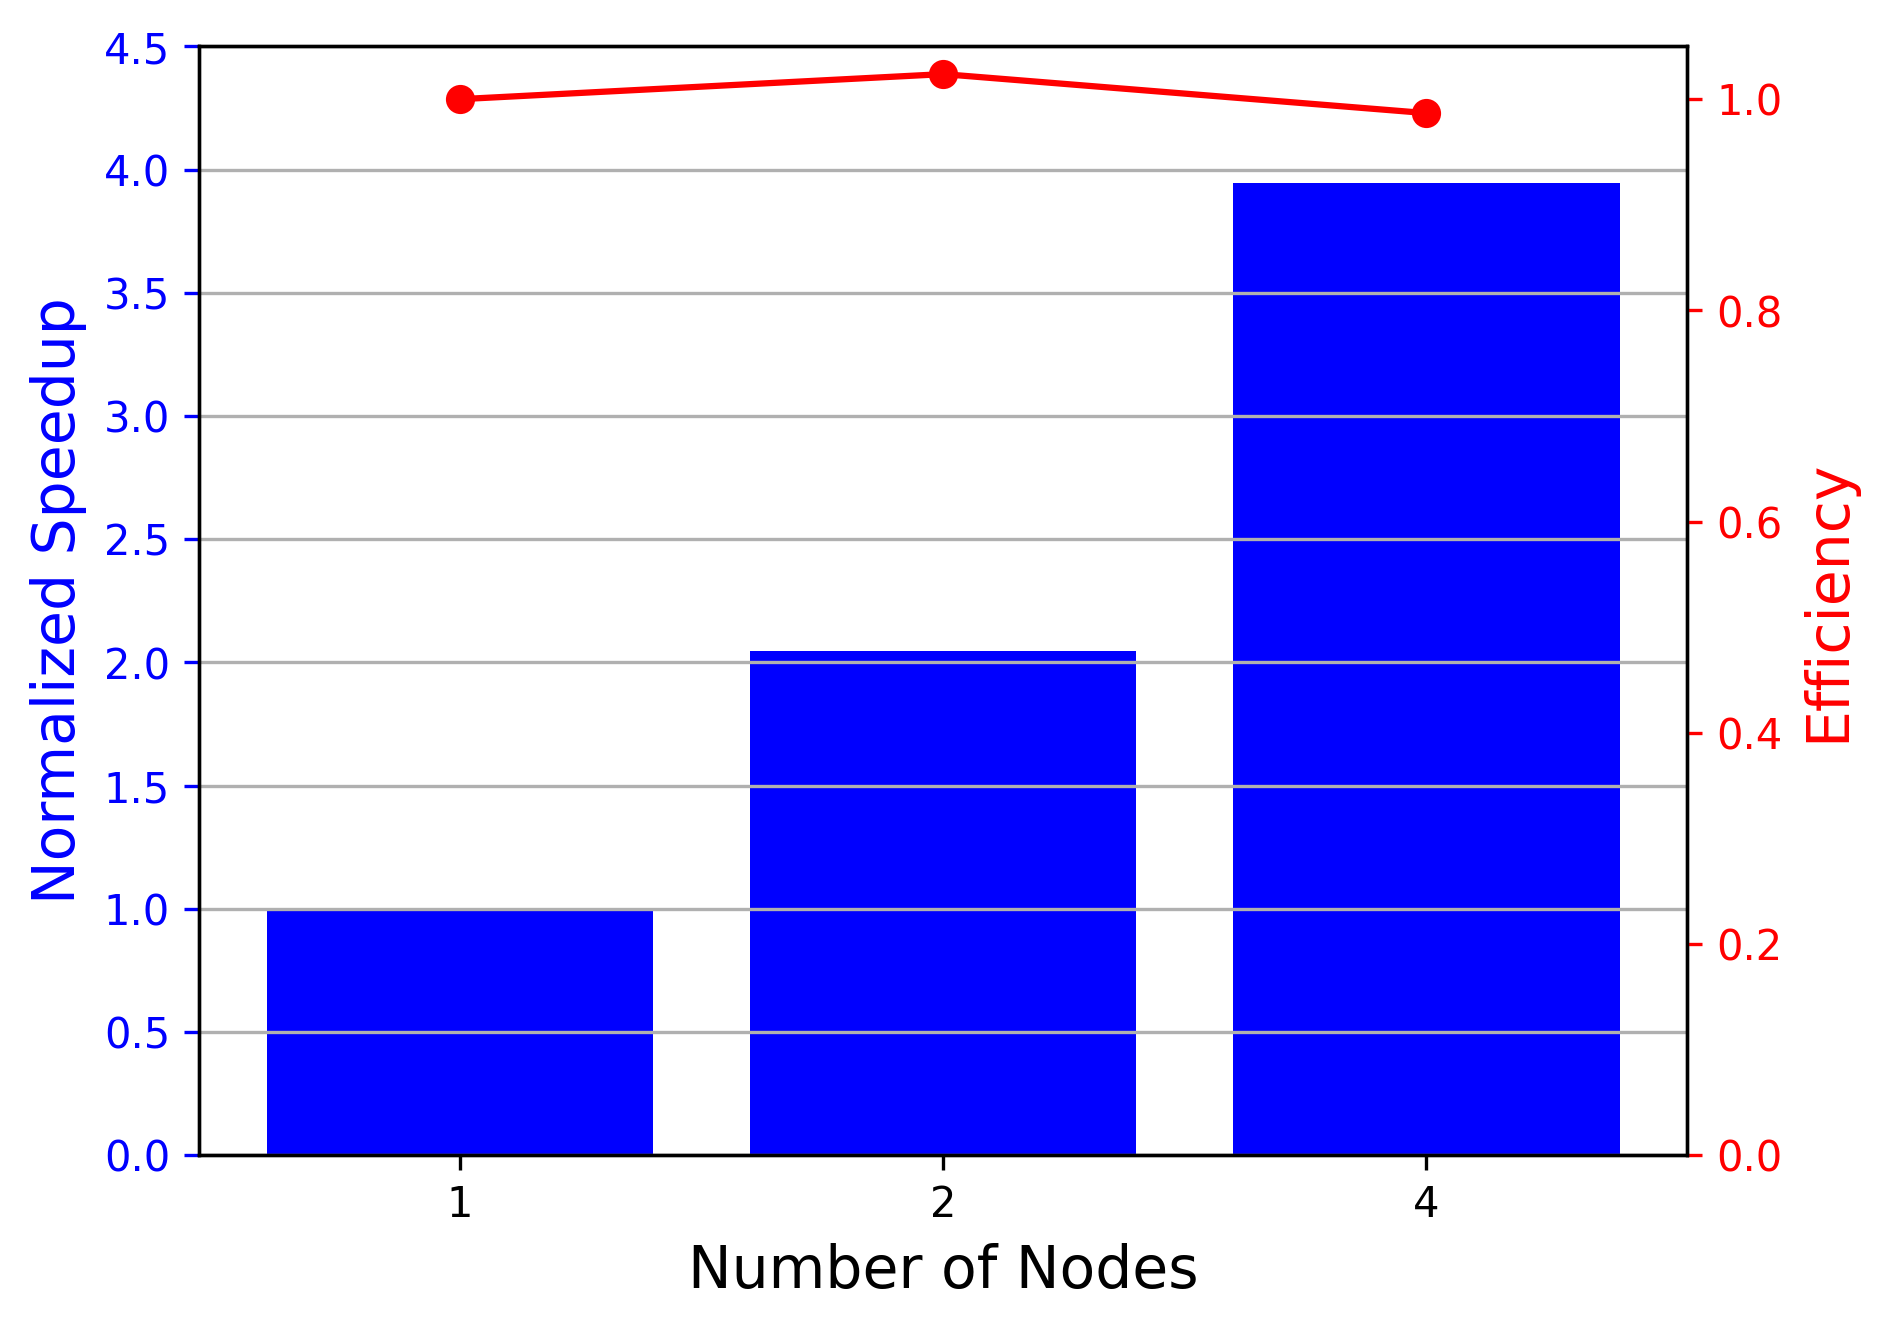
\includegraphics[width=.9\textwidth]{figs/final_optimized.png}
            \caption{CUDA-Aware MPI - Final performance}
            \end{figure}
        \end{minipage}
    \end{columns}
    

    %  synchGhostLayerAfterWrite(); 
    %  synchCopyLayerBeforeRead() 
    
    \end{frame}



%%%%%%%%%%%%%%%%%%%%%%%%%%%%%%%%%%%%%%%%%%%%%%%%%%%%%%%%%%%%%%%%%%%%%%%%%%%%%%%

% \\begin{table}[h!]
% 	\centering
%   \begin{tabular}{ |p{5cm}|p{3cm}|p{3cm}|p{3cm}|p{3cm}|}
% 	\hline
% 		  							& normal CUDA+MPI & CUDA-Aware-MPI &  CUDA-Aware-MPI With Data Packing  	\\
% 	\hline
% 	cpu time(s)                 & 3.26161     & 5.26526 				  & 4.2443 							\\
% 	\hline
% 	cpu+comm time(s)                  & 3.32326     &  304.851 				  & 5.169			 	\\
% 	\hline
% 	cuMemcpyAsync(ns)		& 42752677     & 223807195575 				  & 60358765					\\
% 	\hline
% 	cuStreamSynchorize(ns) &1432637476  & 96648603117 & 22810017\\
% 	\hline
% 	cudaDeviceSynchronize(ns) &0  & 4027609708 & 3408322468\\
% 	\hline
% 	computeNetUpdateKernel(ns) & 1441814837 & 2463512371 & 1456333225\\
% 	\hline
% 	cuda memcpy HtoD(ns) & 39646099 & 34546762344 & 5375257\\
% 	\hline
% 	MPI Sendrecv(ns) & 102990405 & 392695201813 & 1294693583\\
% 	\hline
%   \end{tabular}
%   \caption{Profiling Data Comparison(4MPI,x,y=4096): CUDA+MPI vs. CUDA-Aware-MPI vs. CUDA-Aware-MPI with Data Packing}
%   \label{table:opt_profile}
% \end{table}


\end{document}
